\documentclass[a4paper]{article}
\usepackage{vntex}
%\usepackage[english,vietnam]{babel}
%\usepackage[utf8]{inputenc}

%\usepackage[utf8]{inputenc}
%\usepackage[francais]{babel}
\usepackage{a4wide,amssymb,epsfig,latexsym,array,hhline,fancyhdr}
\usepackage[normalem]{ulem}
%\usepackage{soul}

\usepackage[makeroom]{cancel}
\usepackage{amsmath}
\usepackage{amsthm}
\usepackage{multicol,longtable,amscd}
\usepackage{diagbox}%Make diagonal lines in tables
\usepackage{booktabs}
\usepackage{alltt}
\usepackage[framemethod=tikz]{mdframed}% For highlighting paragraph backgrounds
\usepackage{caption,subcaption}

\usepackage{lastpage}
\usepackage[lined,boxed,commentsnumbered]{algorithm2e}
\usepackage{enumerate}
\usepackage{color}
\usepackage{graphicx}							% Standard graphics package
\usepackage{array}
\usepackage{tabularx, caption}
\usepackage{multirow}
\usepackage{multicol}
\usepackage{rotating}
\usepackage{graphics}
\usepackage{geometry}
\usepackage{setspace}
\usepackage{epsfig}
\usepackage{tikz}
\usetikzlibrary{arrows,snakes,backgrounds}
\usepackage[unicode]{hyperref}
\hypersetup{urlcolor=blue,linkcolor=black,citecolor=black,colorlinks=true} 
%\usepackage{pstcol} 								% PSTricks with the standard color package

\usepackage[normalem]{ulem}

\newtheorem{theorem}{{\bf Định lý}}
\newtheorem{property}{{\bf Tính chất}}
\newtheorem{proposition}{{\bf Mệnh đề}}
\newtheorem{corollary}[proposition]{{\bf Hệ quả}}
\newtheorem{lemma}[proposition]{{\bf Bổ đề}}
\theoremstyle{definition}
\newtheorem{exer}{Bài toán}

\def\thesislayout{	% A4: 210 × 297
	\geometry{
		a4paper,
		total={160mm,240mm},  % fix over page
		left=30mm,
		top=30mm,
	}
}
\thesislayout

%\usepackage{fancyhdr}
\setlength{\headheight}{40pt}
\pagestyle{fancy}
\fancyhead{} % clear all header fields
\fancyhead[L]{
 \begin{tabular}{rl}
    \begin{picture}(25,15)(0,0)
    \put(0,-8){
\includegraphics[width=8mm, height=8mm]{Images/hcmut.png}}
    %\put(0,-8){\epsfig{width=10mm,figure=hcmut.eps}}
   \end{picture}&
	%
\includegraphics[width=8mm, height=8mm]{hcmut.png} & %
	\begin{tabular}{l}
		\textbf{\bf \ttfamily Trường Đại Học Bách Khoa Tp.Hồ Chí Minh}\\
		\textbf{\bf \ttfamily Khoa Khoa Học \& Kỹ Thuật Máy Tính}
	\end{tabular} 	
 \end{tabular}
}
\fancyhead[R]{
	\begin{tabular}{l}
		\tiny \bf \\
		\tiny \bf 
	\end{tabular}  }
\fancyfoot{} % clear all footer fields
\fancyfoot[L]{\scriptsize \ttfamily Đề bài tập lớn môn Cấu trúc Rời rạc cho KHMT (CO1007) - Niên khóa 2021-2022}
\fancyfoot[R]{\scriptsize \ttfamily Trang {\thepage}/\pageref{LastPage}}
\renewcommand{\headrulewidth}{0.3pt}
\renewcommand{\footrulewidth}{0.3pt}


%%%
\setcounter{secnumdepth}{4}
\setcounter{tocdepth}{3}
\makeatletter
\newcounter {subsubsubsection}[subsubsection]
\renewcommand\thesubsubsubsection{\thesubsubsection .\@alph\c@subsubsubsection}
\newcommand\subsubsubsection{\@startsection{subsubsubsection}{4}{\z@}%
                                     {-3.25ex\@plus -1ex \@minus -.2ex}%
                                     {1.5ex \@plus .2ex}%
                                     {\normalfont\normalsize\bfseries}}
\newcommand*\l@subsubsubsection{\@dottedtocline{3}{10.0em}{4.1em}}
\newcommand*{\subsubsubsectionmark}[1]{}
\makeatother

\everymath{\color{blue}}%make in-line maths symbols blue to read/check easily

\sloppy
\captionsetup[figure]{labelfont={small,bf},textfont={small,it},belowskip=-1pt,aboveskip=-9pt}
%space remove between caption, figure, and text
\captionsetup[table]{labelfont={small,bf},textfont={small,it},belowskip=-1pt,aboveskip=7pt}
%space remove between caption, table, and text

%\floatplacement{figure}{H}%forced here float placement automatically for figures
%\floatplacement{table}{H}%forced here float placement automatically for table
%the following settings (11 lines) are to remove white space before or after the figures and tables
%\setcounter{topnumber}{2}
%\setcounter{bottomnumber}{2}
%\setcounter{totalnumber}{4}
%\renewcommand{\topfraction}{0.85}
%\renewcommand{\bottomfraction}{0.85}
%\renewcommand{\textfraction}{0.15}
%\renewcommand{\floatpagefraction}{0.8}
%\renewcommand{\textfraction}{0.1}
\setlength{\floatsep}{5pt plus 2pt minus 2pt}
\setlength{\textfloatsep}{5pt plus 2pt minus 2pt}
\setlength{\intextsep}{10pt plus 2pt minus 2pt}

\thesislayout
\begin{document}

\begin{titlepage}
\begin{center}
ĐẠI HỌC QUỐC GIA THÀNH PHỐ HỒ CHÍ MINH \\
TRƯỜNG ĐẠI HỌC BÁCH KHOA \\
KHOA KHOA HỌC \& KỸ THUẬT MÁY TÍNH 
\end{center}

\vspace{1cm}

\begin{figure}[h!]
\begin{center}

\includegraphics[width=3cm]{Images/hcmut.png}
\end{center}
\end{figure}

\vspace{1cm}


\begin{center}
\begin{tabular}{c}
\multicolumn{1}{l}{\textbf{{\Large CẤU TRÚC RỜI RẠC CHO KHMT (CO1007)}}}\\
~~\\
\hline
\\
% \multicolumn{1}{l}{\textbf{{\Large Đề bài tập lớn cho Nhóm $n$}}}\\
% \\
% \textbf{{\Huge Thống kê mô tả và}} \\
% \textbf{{\Huge Xác suất rời rạc với R}}\\
\textbf{\large Thống kê khảo sát kết quả Covid-19}\\
\textbf{\large môn Cấu trúc rời rạc}
\\
\hline
\end{tabular}
\end{center}

\vspace{1.5cm}

\begin{table}[h]
\begin{tabular}{rrl}
\hspace{5 cm} & GVHD: & Huỳnh Tường Nguyên\\
\hspace{5 cm} &  & Nguyễn Ngọc Lễ\\

& SV thực hiện: & Võ Tấn Hưng -- 2113623 \\
& & Trương Thuận Hưng -- 2113619 \\
& & Đỗ Minh Đức -- 2113206 \\
& & Nguyễn Hoàng Kim -- 2111617 \\
& & Nguyễn Phạm Thiên Phúc -- 2114445 \\
& & Vũ Xuân Mai Trung -- 2115129 \\
\end{tabular}
\end{table}
\vspace{1.5cm}
\begin{center}
{\footnotesize Tp. Hồ Chí Minh, Tháng 04/2022}
\end{center}
\end{titlepage}
\pagebreak

\begin{enumerate}[i)]
\item \textcolor{red}{Nhóm câu hỏi liên quan đến tổng quát dữ liệu}
\begin{enumerate}[1)]
    \item Tập mẫu thể hiện thu thập dữ liệu vào các năm:\textcolor{blue} {2020; 2021; 2022}
    \item Số lượng đất nước và định danh của mỗi đất nước (hiển thị 10 đất nước đầu tiên).
    \begin{center}
      \begin{tabular}{ c  l  }
    iso\_code: & Country              \\  
    ABW      &    Aruba               \\            
    AFG      &   Afghanistan          \\        
    AGO      &    Angola              \\        
    AIA      &    Anguilla            \\       
    ALB      &    Albania             \\         
    AND      &    Andorra             \\        
    ARE      &    United Arab Emirates\\
    ARG      &    Argentina           \\
    ARM      &    Armenia             \\
    ATG      &    Antigua and Barbuda \\  
    Count    &    225                 
       \end{tabular}
    \end{center}
    \item Số lượng châu lục trong tập mẫu
    \begin{center}
      \begin{tabular}{ c l }
        Continent:  &            6      \\
          Asia:      &   Châu Á         \\
        Europe:     &  Châu Âu          \\
        Africa:      & Châu Phi         \\
 North America:      &   Bac Mi         \\
 South America:      &   Nam Mi         \\
       Oceania:      & Chau Dai Duong   
       \end{tabular}
    \end{center}
    \item Số lượng dữ liệu thể hiện thu thập dữ liệu được trong từng từng châu lục và tổng số
    \begin{center}
      \begin{tabular}{ c l }
      Continent: &    Observations \\
      Africa     &        38647    \\  
      Asia       &        35528    \\   
      Europe     &        36375    \\   
   North America &        24438    \\   
   Oceania       &        8993     \\   
   South America &        9335     \\   
   Tong:         &        153316   
     \end{tabular}
    \end{center}
    \item Số lượng dữ liệu thể hiện thu thập dữ liệu được trong từng từng đất nước (hiển thị 10 dất nước cuối cùng) và tổng số
    \begin{center}
      \begin{tabular}{ c l }
iso\_code & Observations \\ 
   VEN &     708         \\
   VGB &     694         \\
   VNM &     759         \\
   VUT &     467         \\
   WLF &     489         \\
   WSM &     459         \\
   YEM &     681         \\
   ZAF &     744         \\ 
   ZMB &     704         \\
   ZWE &     702         \\
 Tong: &   153316  
      \end{tabular}
    \end{center}
    \item Các châu lục nào có lượng dữ liệu thu thập nhỏ nhất và giá trị nhó nhất
    \begin{center}
      \begin{tabular}{ c l }
  Continent:  & Minimum   \\
   Oceania:   &      8993
      \end{tabular}
    \end{center}
    \item Các châu lục nào có lượng dữ liệu thu thập lớn nhất và giá trị lớn nhất 
    \begin{center}
      \begin{tabular}{ c l }
  Continent:  & Maximum   \\
   Africa:     &    38647
      \end{tabular}
    \end{center}
    \item Các nước nào có lượng dữ liệu thu thập nhỏ nhất và giá trị nhó nhất 
    \begin{center}
      \begin{tabular}{ c l }
  Country:  & Minimum   \\
  Pitcairn: &   85
      \end{tabular}
    \end{center}
    \item Các nước nào có lượng dữ liệu thu thập lớn nhất và giá trị lớn nhất 
    \begin{center}
      \begin{tabular}{ c l }
  Country   & Maximum   \\
 Argentina: &     781   \\
 Mexico   : &     781
      \end{tabular}
    \end{center}
    \item Các date nào có lượng dữ liệu thu thập nhỏ nhất và giá trị nhó nhất 
    \begin{center}
      \begin{tabular}{ c l }
  Date:      & Minumum  \\
  1/1/2020   &    2     \\
  1/2/2020   &    2     \\
  1/3/2020   &    2    
       \end{tabular}
    \end{center}
    \item Các date nào có lượng dữ liệu thu thập lớn nhất và giá trị lớn nhất 
    \begin{center}
      \begin{tabular}{ c l }
  Date:      & Maximum  \\
  8/22/2021  &   238    \\
  8/23/2021  &   238    \\
  8/24/2021  &   238    \\
  8/25/2021  &   238    \\
  8/26/2021  &   238    \\
  8/27/2021  &   238    \\
  8/28/2021  &   238    \\
  8/29/2021  &   238    
        \end{tabular}
    \end{center}
    \item Dữ liệu thu thập được theo date và châu lục.
    \begin{center}
      \begin{tabular}{ c l l }
    continent & date & numbers of data      \\
  Africa  &  1/1/2021     & 53 \\
  Africa  &  1/1/2022     & 54 \\
  Africa  &  1/10/2021    & 54 \\
  Africa  &  1/10/2022    & 54 \\
  Africa  &  1/11/2021    & 54 \\
  Africa  &  1/11/2022    & 54 \\
  Africa  &  1/12/2021    & 54 \\
  Africa  &  1/12/2022    & 54 \\
  Africa  &  1/13/2021    & 54 \\
  Africa  &  1/13/2022    & 54 \\
  ... with 4,358 more rows 
        \end{tabular}
    \end{center}
    \item Dữ liệu thu thập được là lớn nhất theo date và châu lục: \textcolor{blue} {54} 
    \item Dữ liệu thu thập được là nhỏ nhất theo date và châu lục. \textcolor{blue} {1} 
    \item Dữ liệu thể hiện thu thập dữ liệu duợc ngày 3/23/2020 và châu lục Asia là: \textcolor{blue} {22} 
    \item Các nuớc có số luợng dữ liệu thể hiện thu thập dữ liệu duợc là bằng nhau: \\
    \textcolor{blue} {
       "FJI"      "VNM"      "ABW"      "GIN"      "MLT"      "SOM"      "ATG"      "BLZ"      "HTI"      "MWI"      "BEN"      "BMU"      "BRB"      "ETH"      "LBR"      "SLV"      "TCA"      "GEO"      "KWT"      "LIE"      "TZA"      "KGZ"      "LBY"      "LVA"      "SUR"      "BWA"      "COG"      "OMN"      "ZMB"      "BHS"      "IMN"      "SEN"      "SVK"      "BLR"      "MMR"      "NIC"      "BRN"      "MRT"      "AGO"      "BOL"      "CIV"      "HND"      "MCO"      "MLI"      "NZL"      "SYR"      "ZAF"      "KAZ"      "LKA"      "QAT"      "URY"      "CMR"      "JOR"      "PSE"      "TGO"      "UZB"      "VEN"      "ARM"      "KEN"      "CYP"      "EST"      "MUS"      "NER"      "TTO"      "CPV"      "LTU"      "SAU"      "AFG"      "GMB"      "MNE"      "NGA"      "OWID\_KOS" "ZWE"      "AND"      "BIH"      "CHL"      "COL"      "CZE"      "ISL"      "MKD"      "ROU"      "COD"      "GHA"      "SGP"      "SRB"      "ARE"      "CRI"      "GAB"      "ISR"      "MEX"      "PRY"      "TUN"      "CUW"      "HRV"      "JAM"      "MDA"      "RUS"      "BFA"      "BGD"      "BRA"      "CUB"      "CYM"      "ECU"      "PAK"      "TUR"    "DOM"      "MYS"      "NOR"      "PRT"      "BHR"      "GTM"      "HUN"      "DNK"      "LUX"      "SDN"      "SVN"      "AUT"      "AZE"      "UKR"      "BEL"      "DZA"      "GUY"      "IDN"      "IND"      "IRL"      "PAN"      "POL"      "ALB"      "BGR"      "GRC"      "SWE"      "LBN"      "MAR"      "CAN"      "DEU"      "ARG"      "EGY"      "FIN"      "GBR"      "NLD"      "PER"      "ESP"      "IRQ"      "AUS"      "THA"      "SMR"      "USA"      "FRA"      "IRN"    
    }
    
    \item  iso\_code, tên đất nước mà chiều dài iso\_code lớn hơn 3.
    \begin{center}
      \begin{tabular}{ c l }
   iso\_code & location \\
 OWID\_KOS    & Kosovo 
       \end{tabular}
    \end{center}
    
\end{enumerate}
\item \textcolor{red}{Nhóm câu hỏi liên quan đến mô tả thống kê cơ bản dữ liệu}
 \begin{enumerate}[1)]
 \item Lập bảng mô tả số liệu thống kê cho từng đất nước thuộc về nhóm:
    \begin{figure}[h]
    \centering
    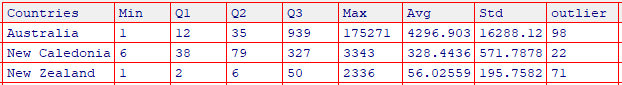
\includegraphics[width=1\textwidth]{Images/bai-2-R-ctotal.png}
    Hình 1: Liên quan về số ca nhiễm
    \end{figure}
    
    \begin{figure}[h]
    \centering
    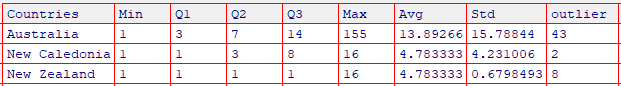
\includegraphics[width=1\textwidth]{Images/bai-2-R-dtotal.png}
    Hình 2: Liên quan về số ca chết
    \end{figure}
 
 \item Vẽ biểu đồ boxplot cho nhiễm coronavirus
    \begin{figure}[h!]
    \centering
    \begin{subfigure}[b]{0.4\linewidth}
    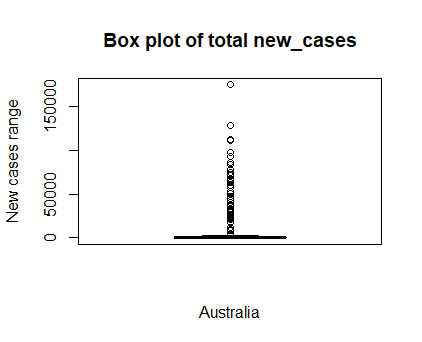
\includegraphics[width=\linewidth]{Images/2-Australia.png}
    \end{subfigure}
    \begin{subfigure}[b]{0.4\linewidth}
    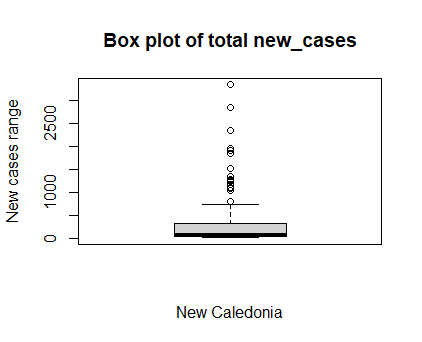
\includegraphics[width=\linewidth]{Images/2-New-Caledonia.png}
    \end{subfigure}
    
    \begin{subfigure}[b]{0.4\linewidth}
    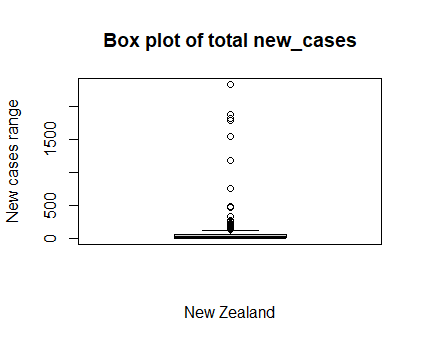
\includegraphics[width=\linewidth]{Images/2-NewZealand.png}
    \end{subfigure}
    \end{figure}
 \end{enumerate}
\item \textcolor{red}{Nhóm câu hỏi liên quan đến dữ liệu thể hiện thu thập dữ liệu}\\
Với mỗi quốc gia mà thuộc về nhóm cần tính số liệu thống kê lần lượt cho nhiễm và tử vong do coronavirus:
 \begin{enumerate}[1)]
 \item Bảng thống kê dữ liệu về số ngày không được báo cáo mới và được báo cáo mới:
 \vspace{1cm}
    \begin{figure}[h]
    \centering
    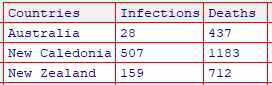
\includegraphics[width=0.5\textwidth]{Images/non-report.png}
    \\Số ngày có số lần dữ liệu không được báo cáo mới
    \end{figure}
    
    \vspace{1cm}
    
    \begin{figure}[h]
    \centering
    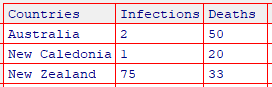
\includegraphics[width=0.5\textwidth]{Images/report-min.png}
    \\Số ngày có số ca nhiễm/tử vong là thấp nhất\\được báo cáo mới
    \end{figure}
    
    \vspace{1cm}
    
    \begin{figure}[h]
    \centering
    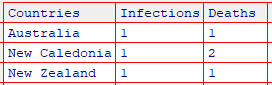
\includegraphics[width=0.5\textwidth]{Images/report-max.png}
    \\Số ngày có số ca nhiễm/tử vong là cao nhất\\được báo cáo mới
    \end{figure}
 \newpage
 \item Bảng thống kê dữ liệu về số ngày liên tiếp không có dữ liệu được báo cáo:
 \vspace{1cm}
    \begin{figure}[h]
    \centering
    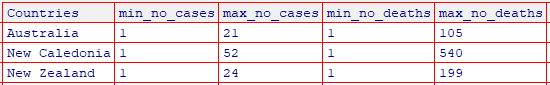
\includegraphics[width=0.75\textwidth]{Images/ex-5-6.png}
    \\Số ngày ngắn nhất/dài nhất liên tiếp\\ mà không có dữ liệu được báo cáo
    \end{figure}
 \vspace{1cm}
 \item Bảng thống kê dữ liệu về số ngày liên tiếp không có người nhiễm bệnh mới:
 \vspace{1cm}
    \begin{figure}[h]
    \centering
    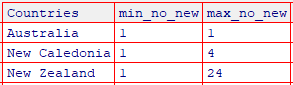
\includegraphics[width=0.5\textwidth]{Images/ex-7-8.png}
    \\Số ngày ngắn nhất/dài nhất liên tiếp\\ mà không có người nhiễm bệnh mới
    \end{figure}
    \end{enumerate}
\item \textcolor{red}{Nhóm câu hỏi liên quan đến trực quan dữ liệu}
\begin{enumerate}[1)]
    \item Vẽ biểu đồ tần số tích lũy quốc gia cho các châu lục
    \begin{figure}[h]
    \centering
    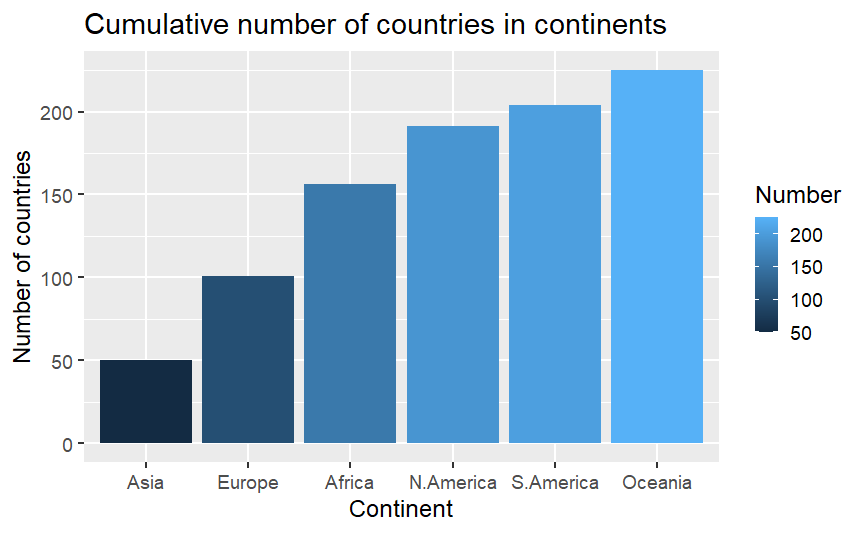
\includegraphics[width=0.5\textwidth]{Images/1iv.png}
    \end{figure}
    \item Vẽ biểu đồ tần số tương đối quốc gia cho các châu lục
    \begin{figure}[h]
    \centering
    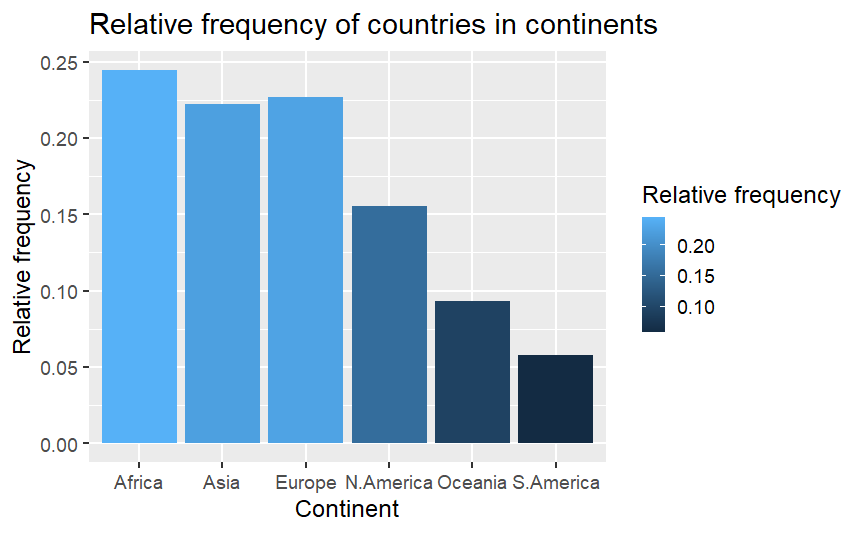
\includegraphics[width=0.5\textwidth]{Images/2iv.png}
    \end{figure}
    \item Vẽ biểu đồ thể hiện nhiễm bệnh đã báo cáo của các quốc gia  mà thuộc về nhóm trong 7 ngày cuối của năm cuối cùng
    \begin{figure}[h]
    \centering
    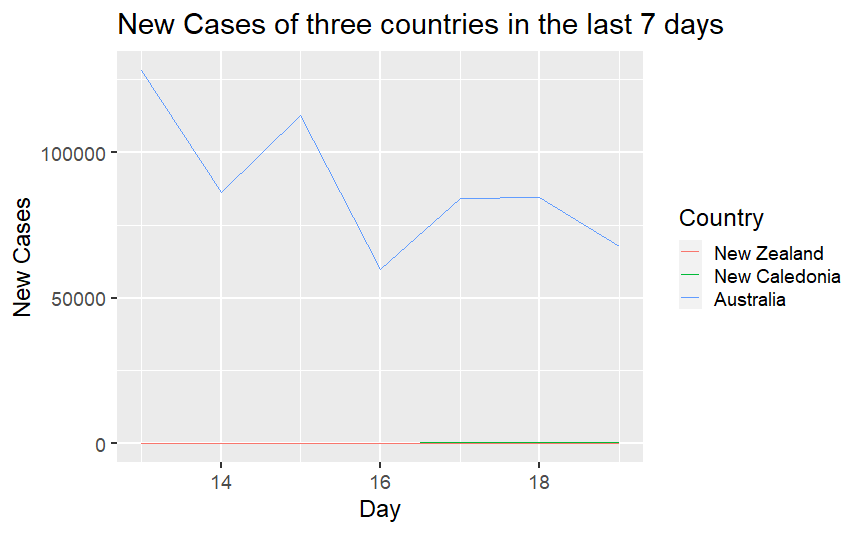
\includegraphics[width=0.5\textwidth]{Images/3iv.png}
    \end{figure}
    \item Vẽ biểu đồ thể hiện tử vong đã báo cáo của các quốc gia  mà thuộc về nhóm trong 7 ngày cuối của năm cuối cùng
    \vspace{5cm}
    \begin{figure}[hpt!]
    \centering
    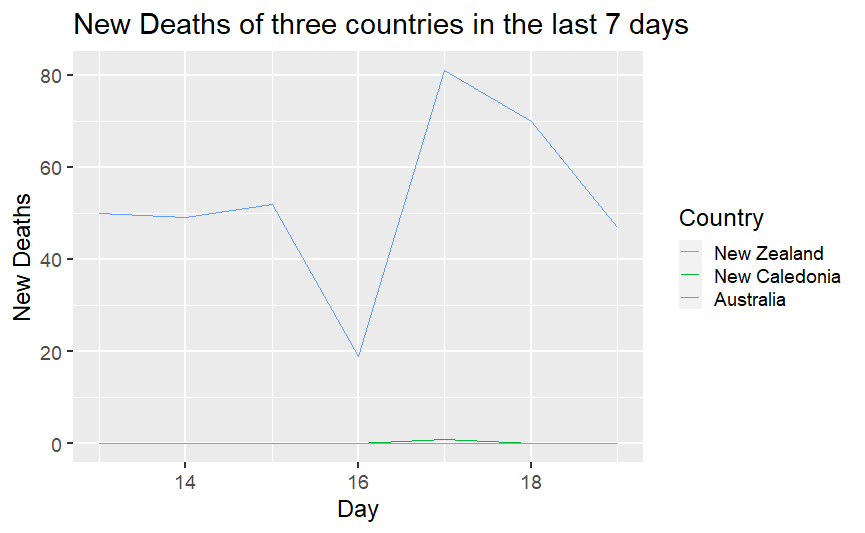
\includegraphics[width=0.5\textwidth]{Images/4ivd.png}
    \end{figure}
    \item Vẽ biểu đồ phổ đất nước xuất hiện outliers cho nhiễm bệnh
    \begin{figure}[hpt!]
    \centering
    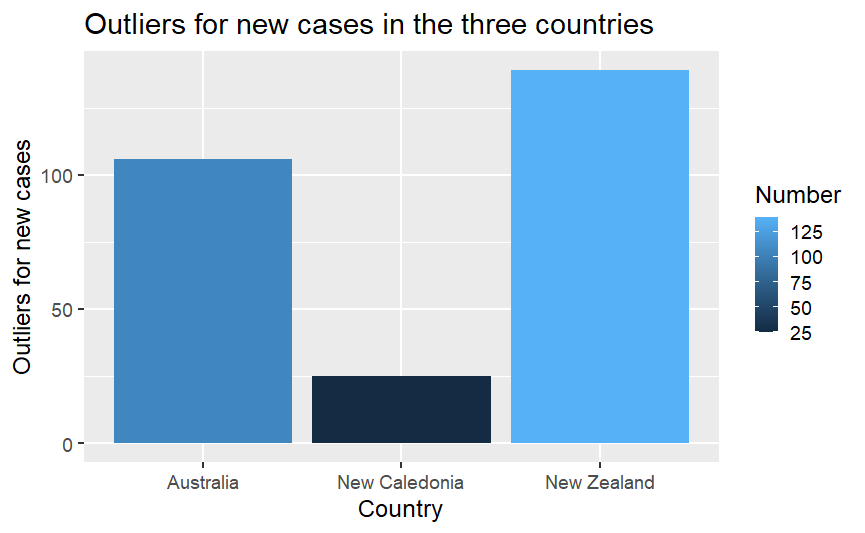
\includegraphics[width=0.5\textwidth]{Images/5iv.png}
    \end{figure}
    \item Vẽ biểu đồ phổ đất nước xuất hiện outliers cho tử vong
    \begin{figure}[hpt!]
    \centering
    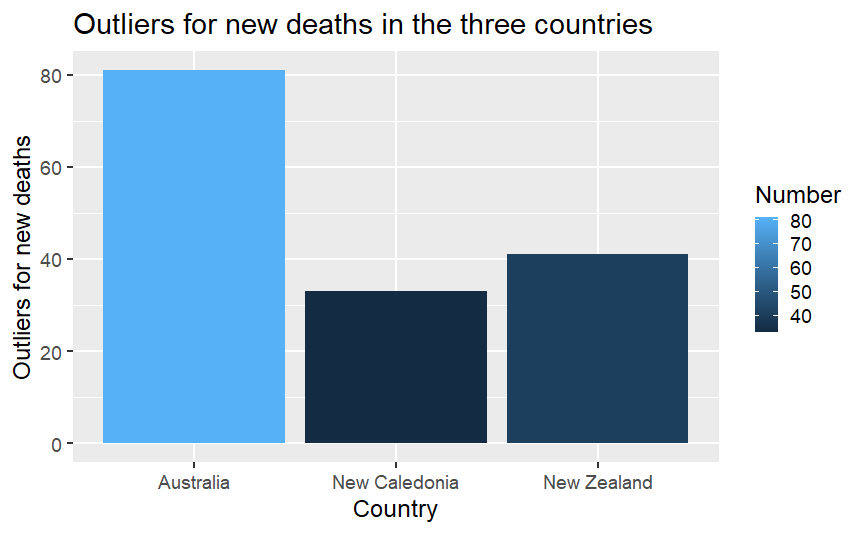
\includegraphics[width=0.5\textwidth]{Images/6iv.png}
    \end{figure}
\end{enumerate}
\item \textcolor{red}{Nhóm câu hỏi liên quan đến trực quan dữ liệu theo thời gian là tháng}\\
Với mỗi quốc gia mà thuộc về nhóm, trên từng năm hãy vẽ biểu đồ thể hiện trục Ox là thời gian, trục Oy là nhiễm bệnh/tử vong. Hãy dùng 4 ký số của mã đề để vẽ 4 tháng tương ứng theo ký số đó. Nếu ký số là 0 thì lấy tháng là 10.\begin{enumerate}[1]
    \item Biểu đồ thể hiện thu thập dữ liệu nhiễm bệnh cho từng tháng
    
    \begin{itemize}
    \item{Số liệu nhiễm bệnh ở Australia theo từng năm:}
    \vspace{5cm}
    \begin{figure}[hpt!]
    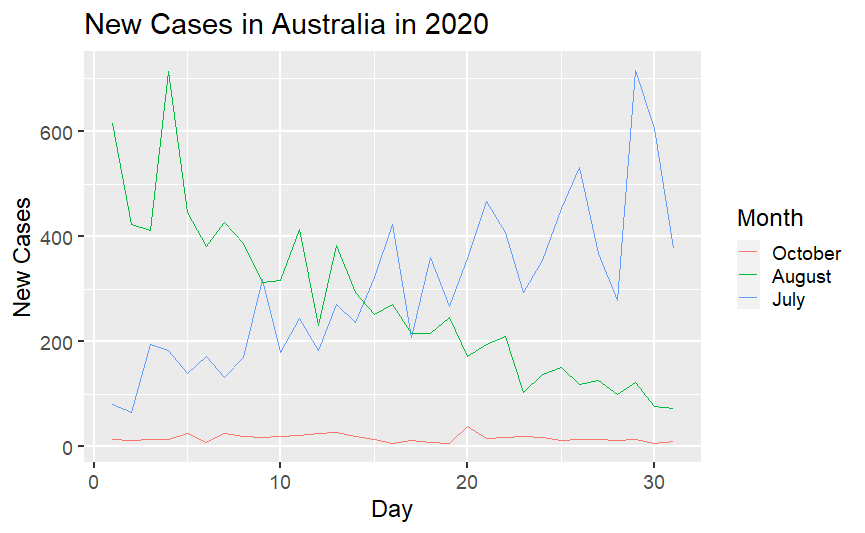
\includegraphics[width=0.5\textwidth]{Images/1.1v.png}
    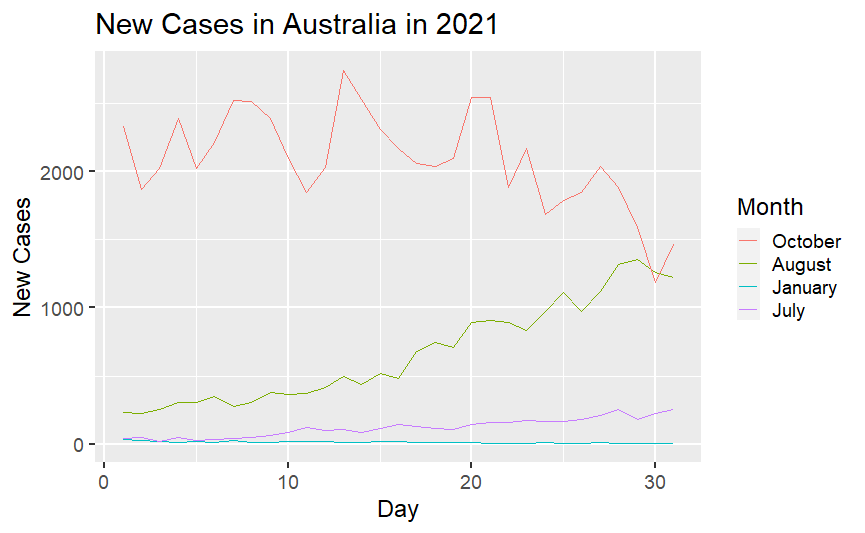
\includegraphics[width=0.5\textwidth]{Images/1.2v.png}
    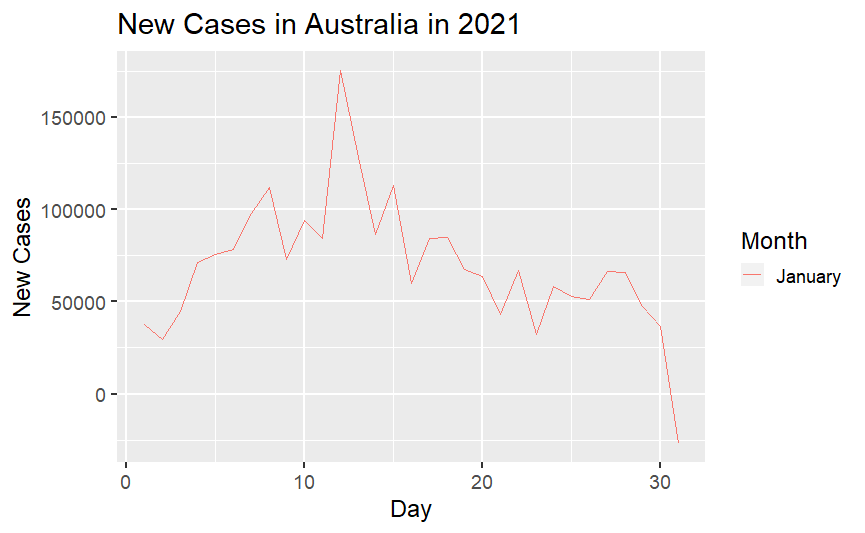
\includegraphics[width=0.5\textwidth]{Images/1.3v.png}
    \end{figure}
    \end{itemize}
    
    \begin{itemize}
   \item{Số liệu nhiễm bệnh ở New Caledonia theo từng năm:}
     \begin{figure}[hpt!]
    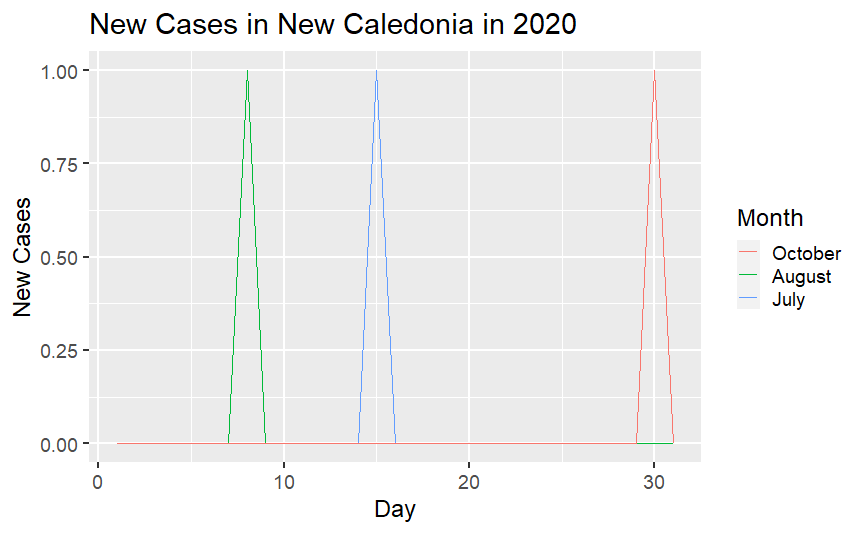
\includegraphics[width=0.5\textwidth]{Images/1.4v.png}
    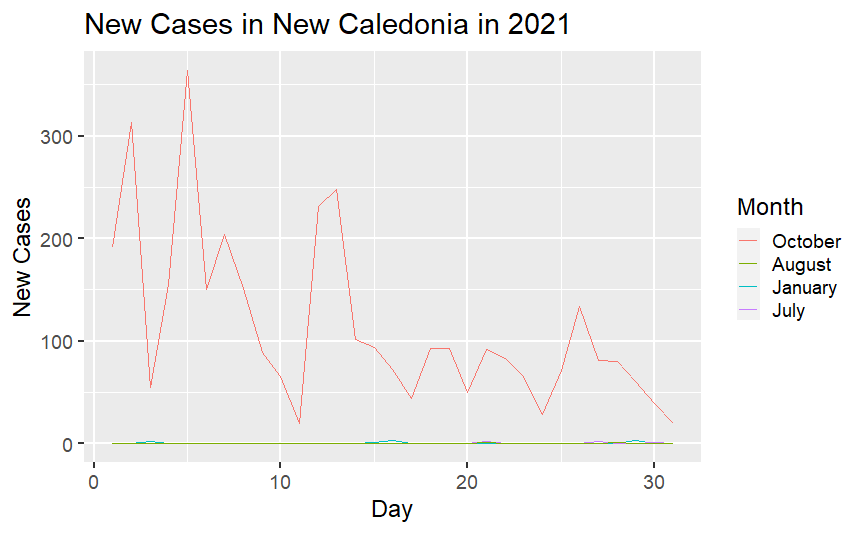
\includegraphics[width=0.5\textwidth]{Images/1.5v.png}
    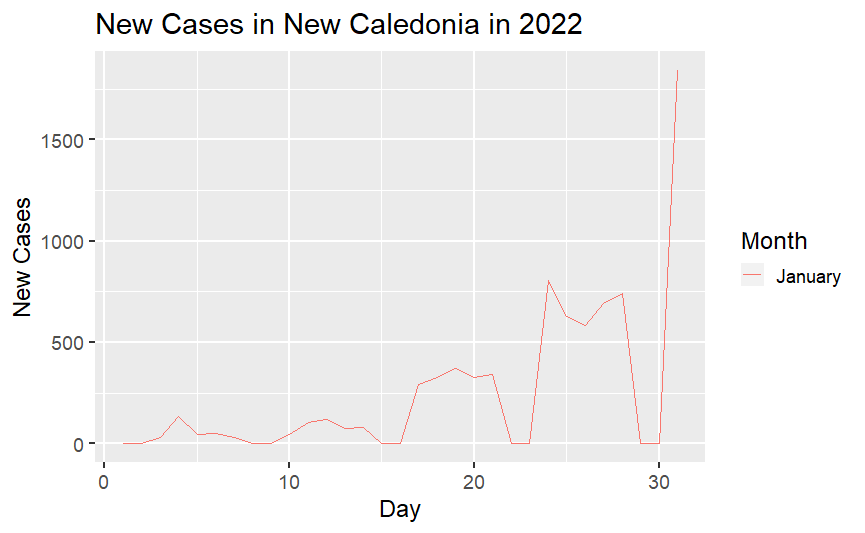
\includegraphics[width=0.5\textwidth]{Images/1.6v.png}
  \end{figure}
    \end{itemize}
    
    \begin{itemize}
   \item{Số liệu nhiễm bệnh ở New Zealand	 theo từng năm:}
     \begin{figure}[hpt!]
    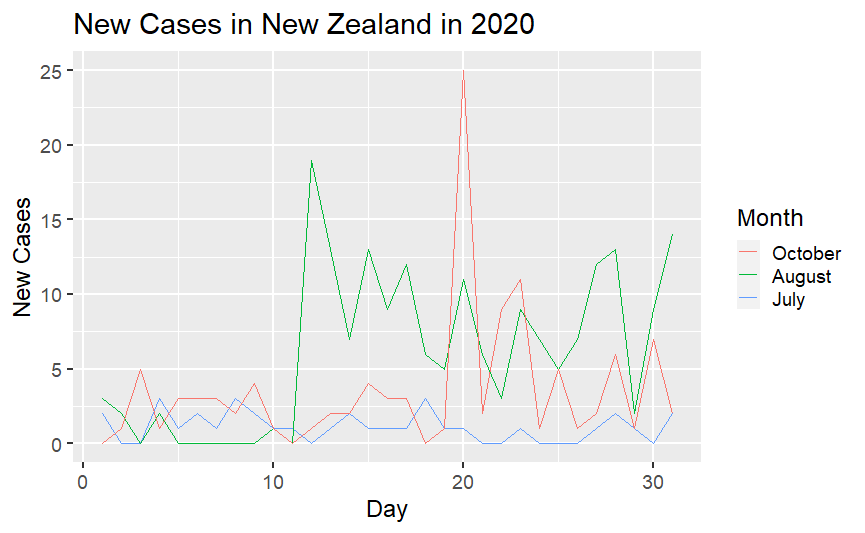
\includegraphics[width=0.5\textwidth]{Images/1.7v.png}
    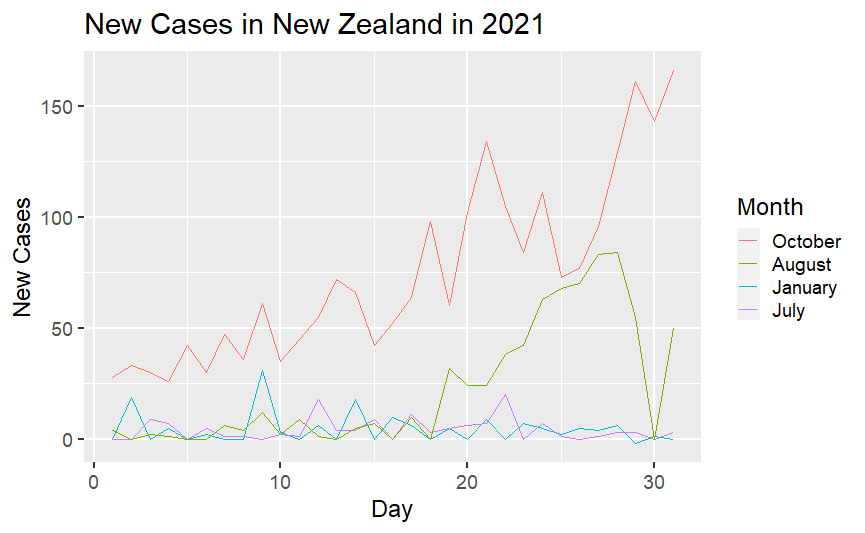
\includegraphics[width=0.5\textwidth]{Images/1.8v.png}
    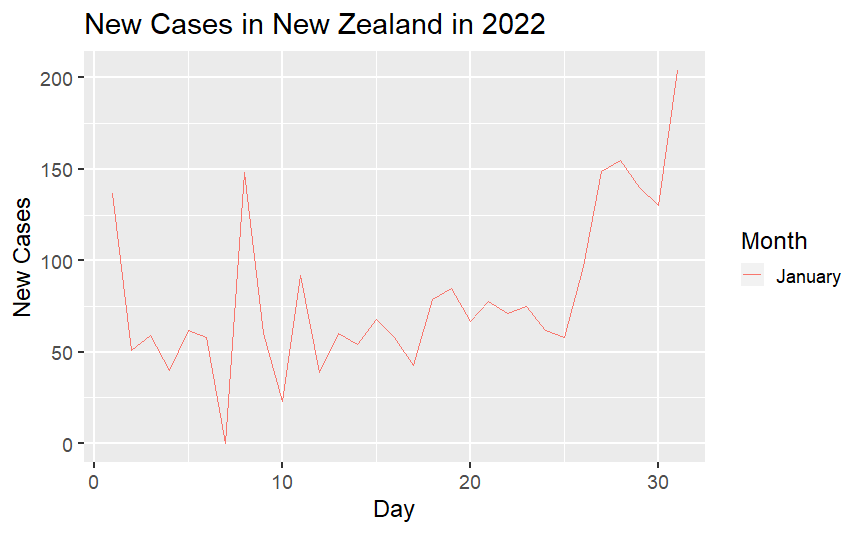
\includegraphics[width=0.5\textwidth]{Images/1.9v.png}
  \end{figure}
    \end{itemize}
   
    \item Biểu đồ thể hiện thu thập dữ liệu tử vong cho từng tháng
    
     \begin{itemize}
   \item{Số liệu tử vong ở Australia theo từng năm:}
  
     \begin{figure}[htp!]
    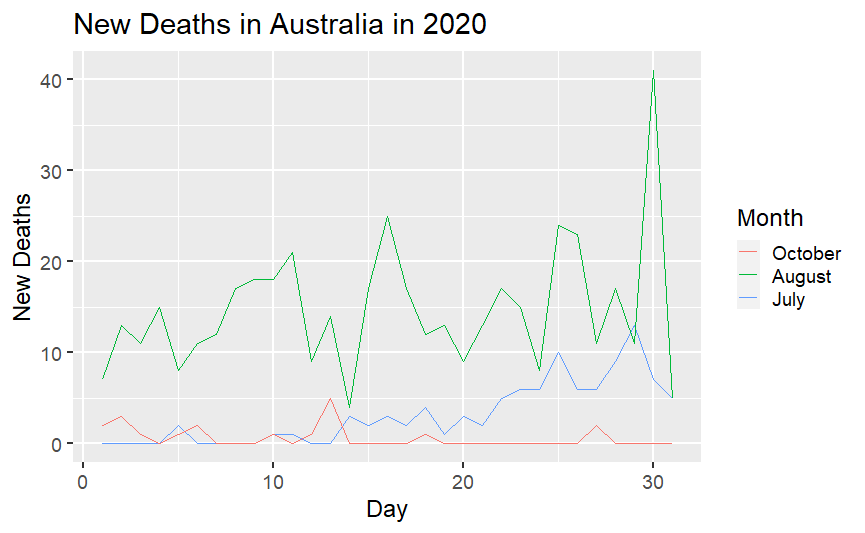
\includegraphics[width=0.5\textwidth]{Images/2.1v.png}
    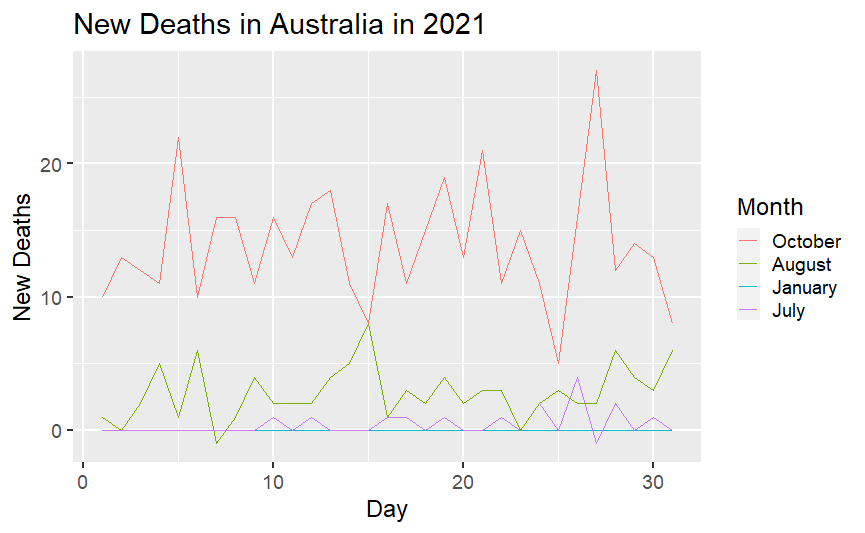
\includegraphics[width=0.5\textwidth]{Images/2.2v.png}
    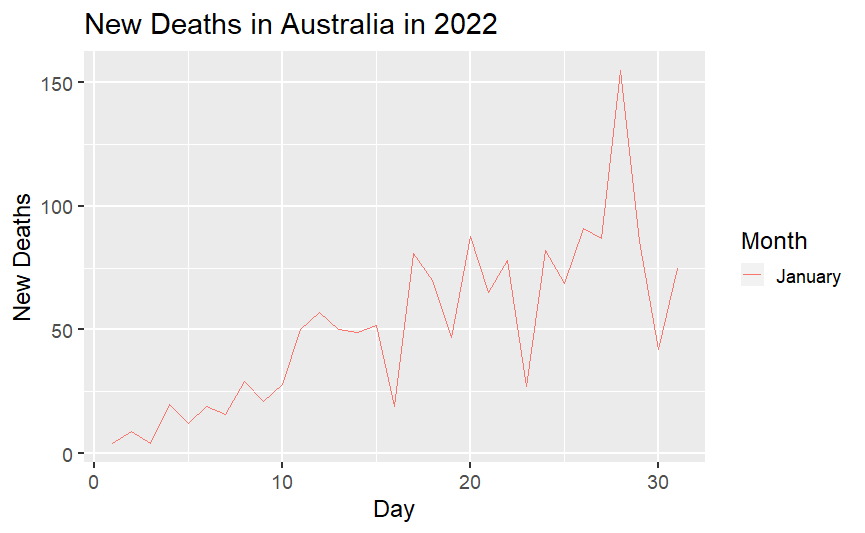
\includegraphics[width=0.5\textwidth]{Images/2.3v.png}
  \end{figure}
    \end{itemize}
    
     \begin{itemize}
   \item{Số liệu tử vong ở New Caledonia theo từng năm:}\\
     \begin{figure}[hpt!]
    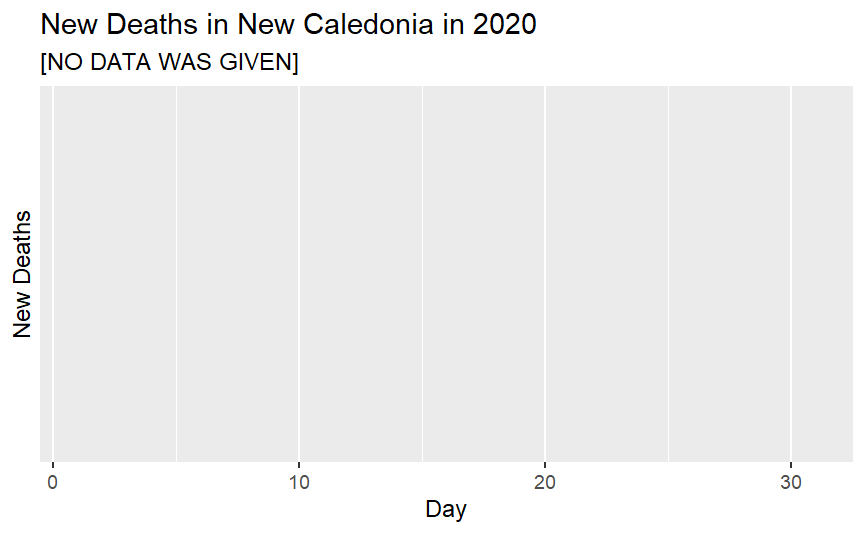
\includegraphics[width=0.5\textwidth]{Images/2.4v.png}
    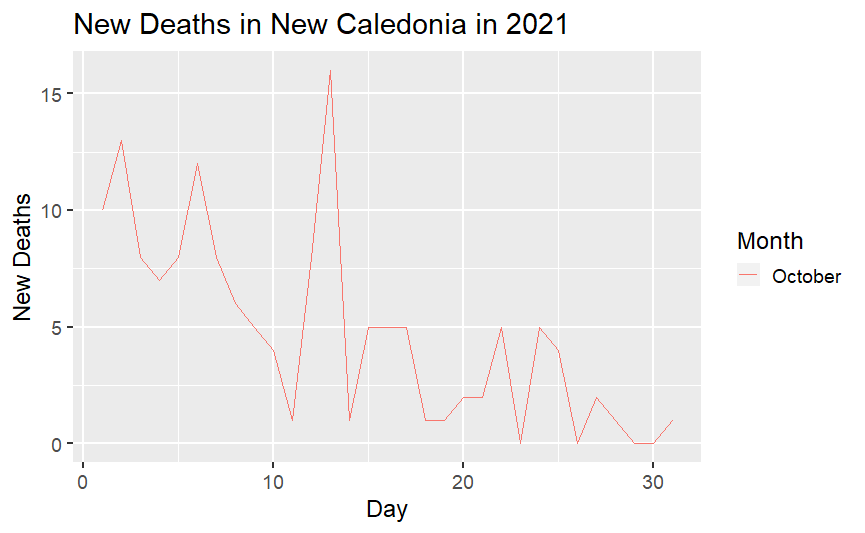
\includegraphics[width=0.5\textwidth]{Images/2.5v.png}
    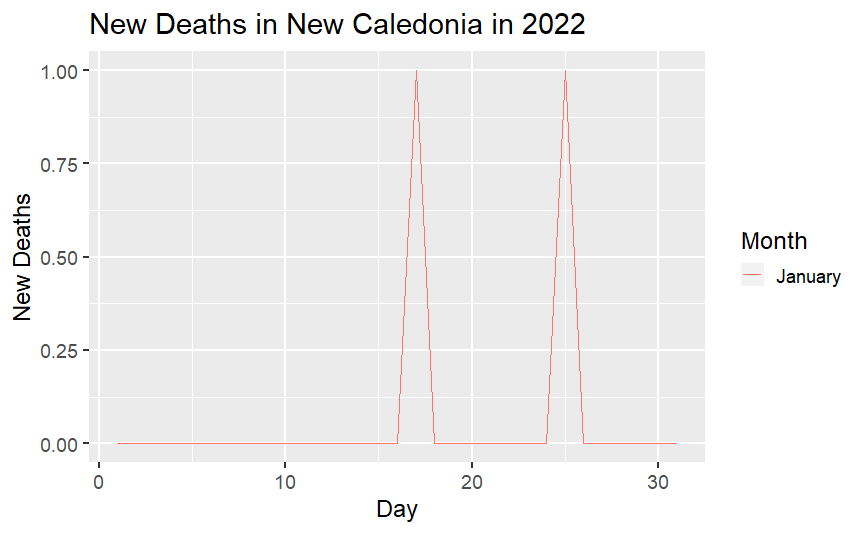
\includegraphics[width=0.5\textwidth]{Images/2.6v.png}
  \end{figure}
    \end{itemize}
    
    \begin{itemize}
   \item{Số liệu tử vong ở New Zealand theo từng năm:}
     \begin{figure}[hpt!]
    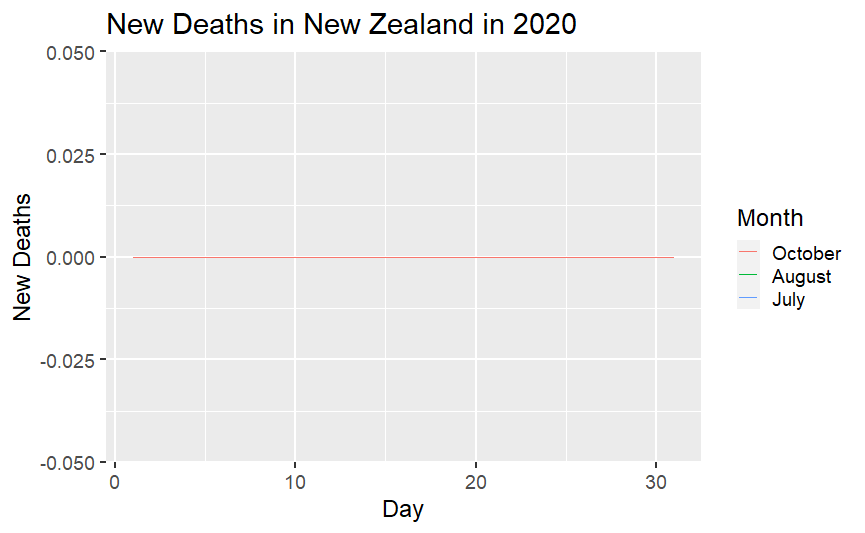
\includegraphics[width=0.49\textwidth]{Images/2.7v.png}
    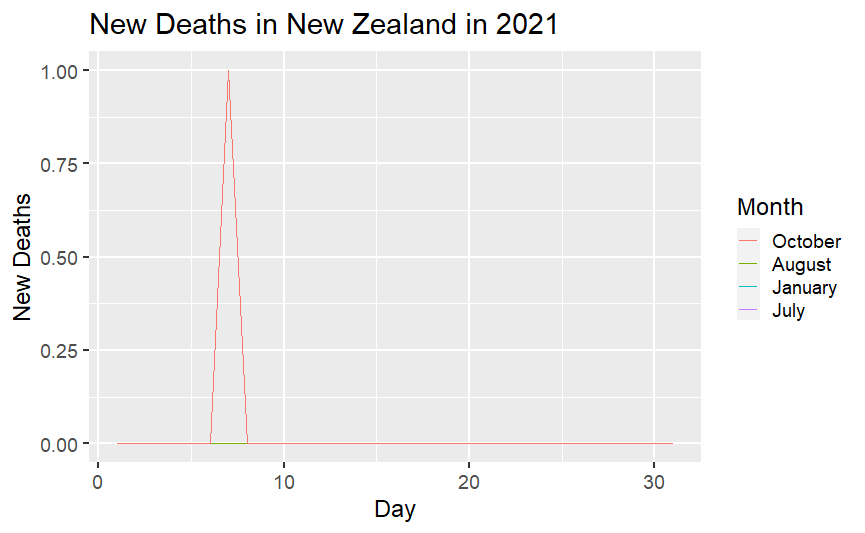
\includegraphics[width=0.49\textwidth]{Images/2.8v.png}
    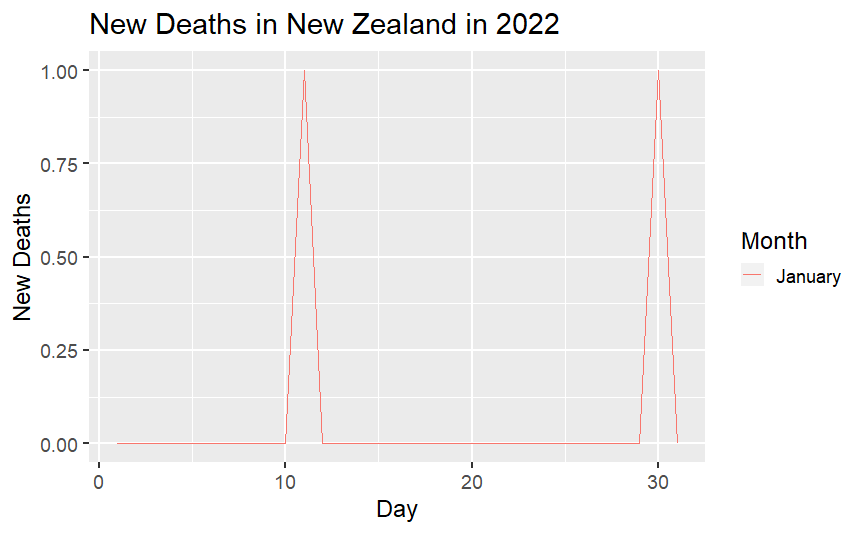
\includegraphics[width=0.49\textwidth]{Images/2.9v.png}
  \end{figure}
    \end{itemize}
    \vspace{10cm}
    \item Biểu đồ thể hiện thu thập dữ liệu gồm nhiễm bệnh và tử vong cho từng tháng 
    
    \begin{itemize}
   \item{Số liệu nhiễm bệnh và tử vong ở Australia theo từng năm:}\\ 
     \begin{figure}[htp!]
    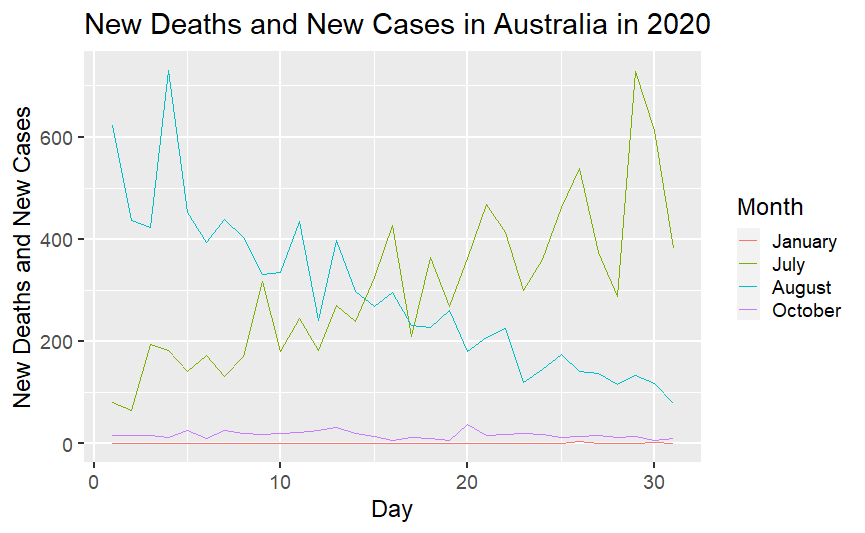
\includegraphics[width=0.48\textwidth]{Images/3.1v.png}
    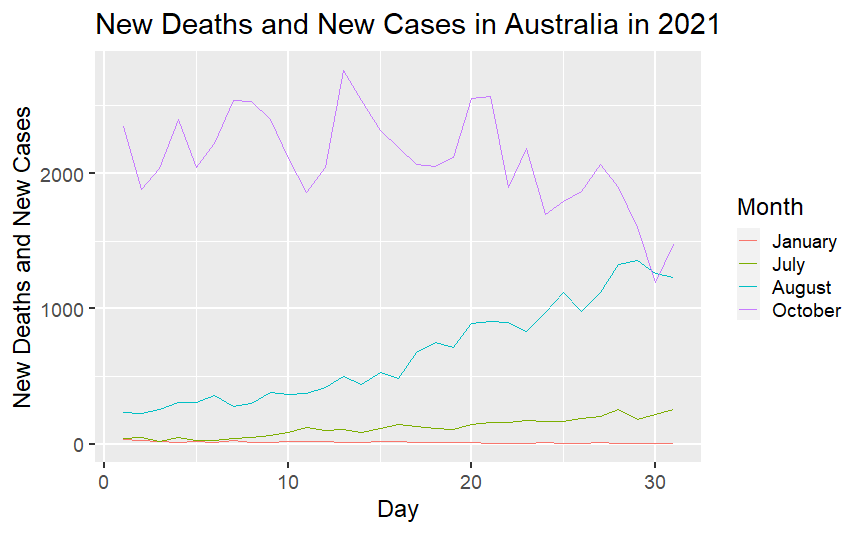
\includegraphics[width=0.48\textwidth]{Images/3.2v.png}
    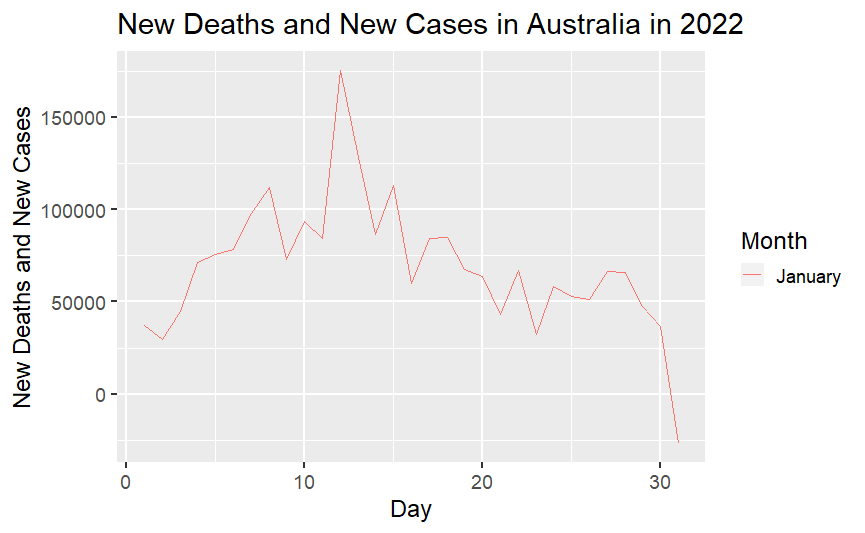
\includegraphics[width=0.48\textwidth]{Images/3.3v.png}
  \end{figure}
    \end{itemize}
    
     \begin{itemize}
    \item{Số liệu nhiễm bệnh và tử vong ở New Caledonia theo từng năm:}\\ 
     \begin{figure}[htp!]
    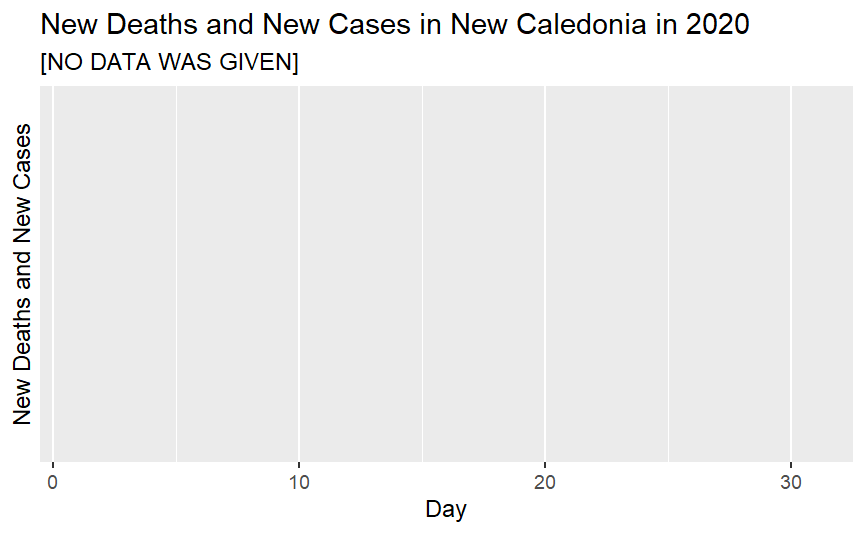
\includegraphics[width=0.45\textwidth]{Images/3.4v.png}
    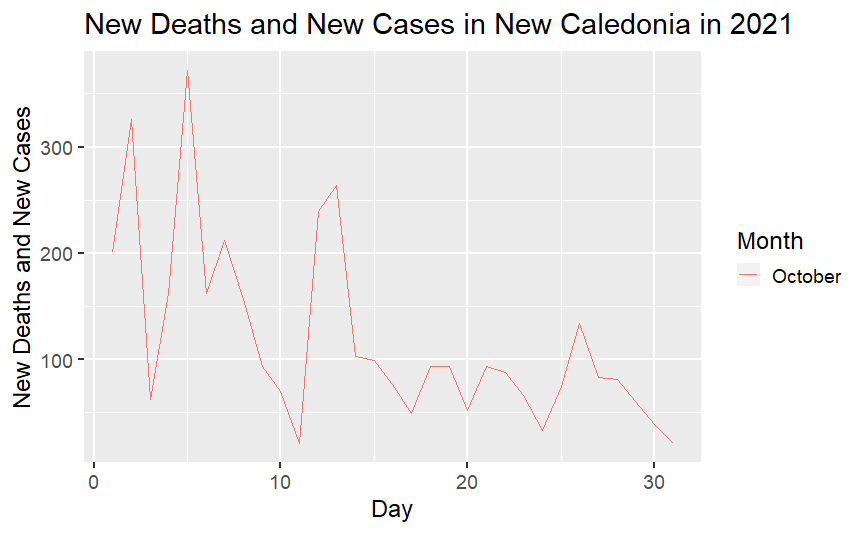
\includegraphics[width=0.45\textwidth]{Images/3.5v.png}
    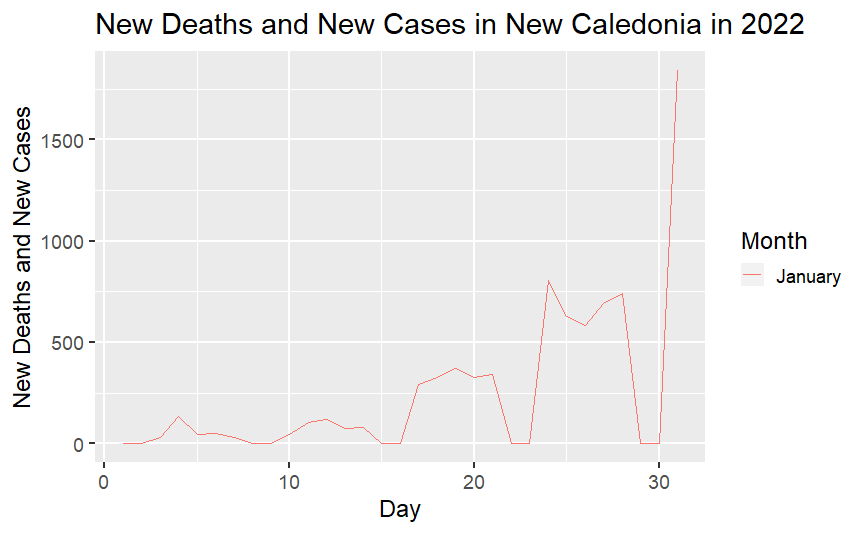
\includegraphics[width=0.45\textwidth]{Images/3.6v.png}
  \end{figure}
    \end{itemize}
    \vspace{5cm}
    
    
     \begin{itemize}
    \item{Số liệu nhiễm bệnh và tử vong ở New Zealand theo từng năm:}\\ 
     \begin{figure}[htp!]
    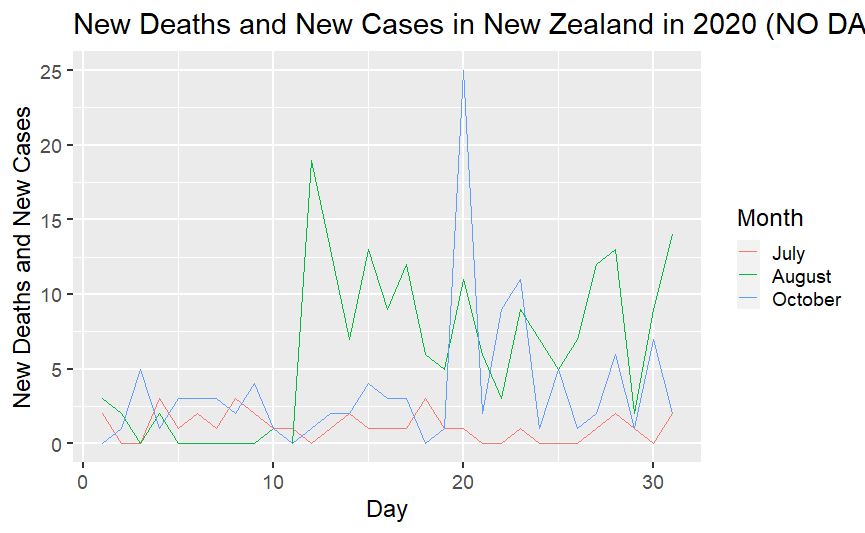
\includegraphics[width=0.5\textwidth]{Images/3.7v.png}
    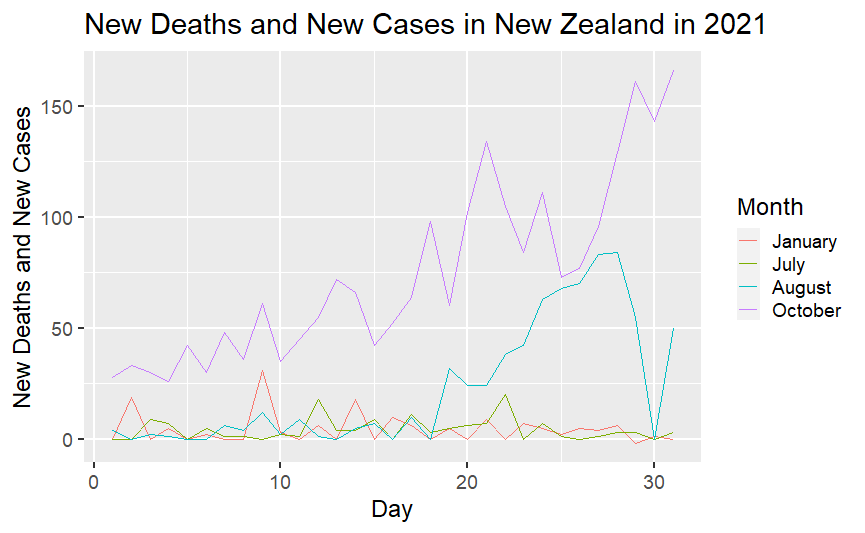
\includegraphics[width=0.5\textwidth]{Images/3.8v.png}
    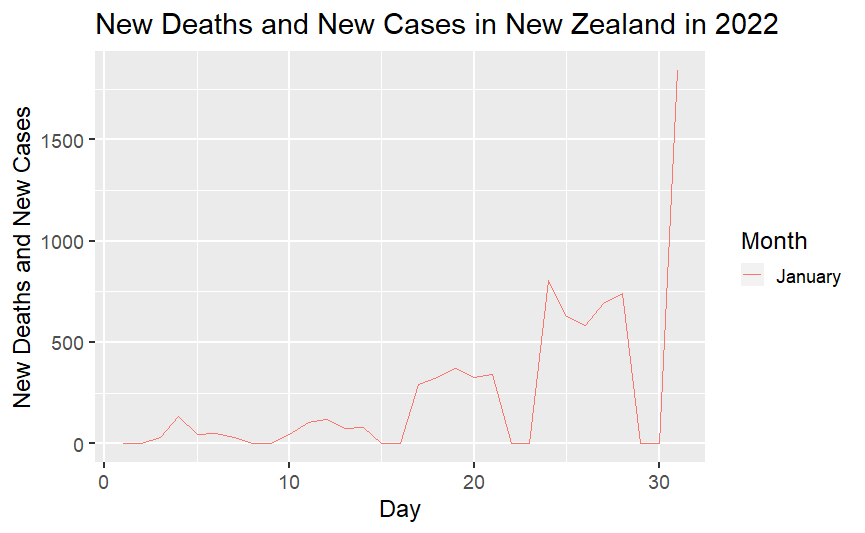
\includegraphics[width=0.5\textwidth]{Images/3.9v.png}
  \end{figure}
    \end{itemize}
    \item Biểu đồ thể hiện thu thập dữ liệu nhiễm bệnh gồm 2 tháng cuối của năm\\
     \begin{itemize}
    \item{Số liệu nhiễm bệnh vào tháng 11 và tháng 12 năm 2020 ở New Zealand, New Caledonia và Australia:}\\ 
     \begin{figure}[htp!]
    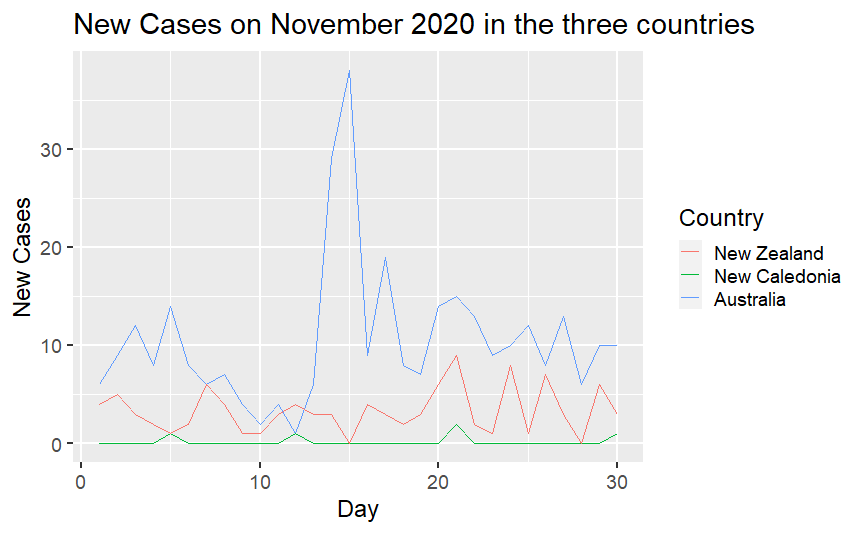
\includegraphics[width=0.5\textwidth]{Images/4.1v.png}
    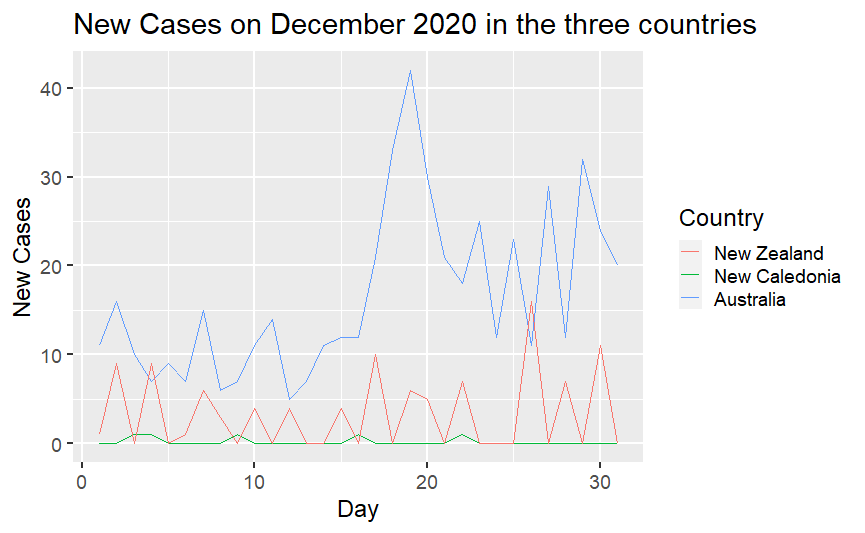
\includegraphics[width=0.5\textwidth]{Images/4.2v.png}
  \end{figure}
    \end{itemize}
    
    \begin{itemize}
    \item{Số liệu nhiễm bệnh vào tháng 11 và tháng 12 năm 2021 ở New Zealand, New Caledonia và Australia:}\\ 
     \begin{figure}[htp!]
    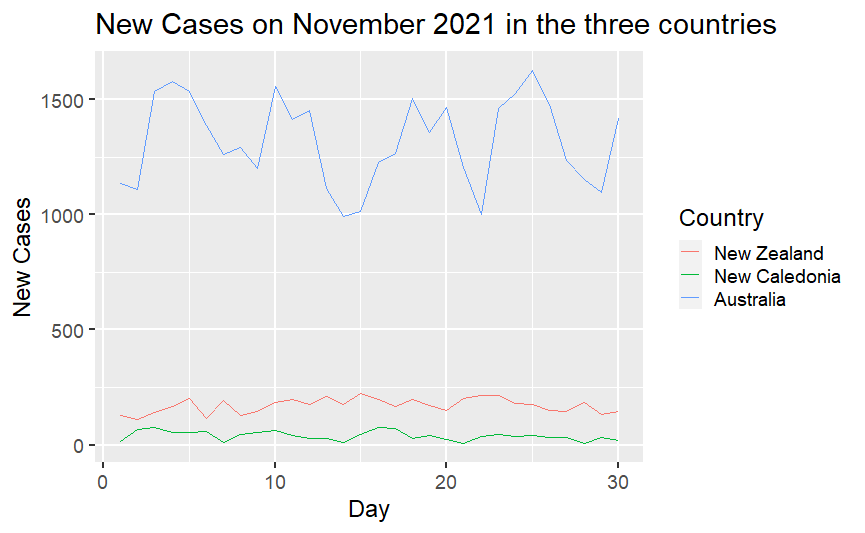
\includegraphics[width=0.5\textwidth]{Images/4.3v.png}
    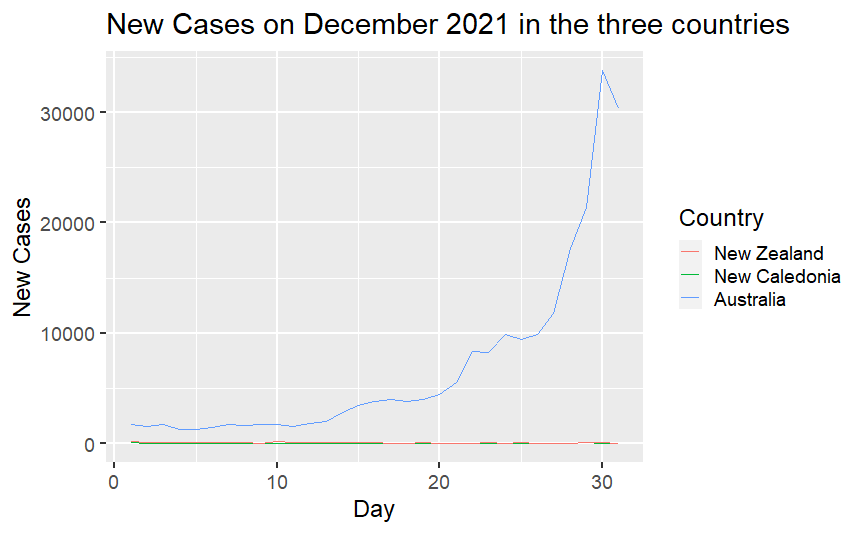
\includegraphics[width=0.5\textwidth]{Images/4.4v.png}
  \end{figure}
    \end{itemize}
    \vspace{10cm}
    \item Biểu đồ thể hiện thu thập dữ liệu tử vong gồm 2 tháng cuối của năm
    \begin{itemize}
    \item{Số liệu tử vong vào tháng 11 và tháng 12 năm 2020 ở New Zealand, New Caledonia và Australia:}\\ 
     \begin{figure}[htp!]
    \includegraphics[width=0.5\textwidth]{Images/5.1v.png}
    \includegraphics[width=0.5\textwidth]{Images/5.2v.png}
  \end{figure}
    \end{itemize}
    
    \begin{itemize}
    \item{Số liệu tử vong vào tháng 11 và tháng 12 năm 2021 ở New Zealand, New Caledonia và Australia:}\\ 
     \begin{figure}[htp!]
    \includegraphics[width=0.5\textwidth]{Images/5.3v.png}
    \includegraphics[width=0.5\textwidth]{Images/5.4v.png}
  \end{figure}
    \end{itemize}
    \vspace{10cm}
    \item Biểu đồ thể hiện thu thập dữ liệu gồm nhiễm bệnh và tử vong gồm 2 tháng cuối của năm
    
    \begin{itemize}
    \item{Số liệu tử vong vào tháng 11 và tháng 12 năm 2020 ở New Zealand, New Caledonia và Australia:}\\ 
     \begin{figure}[htp!]
    \includegraphics[width=0.5\textwidth]{Images/6.1v.png}
    \includegraphics[width=0.5\textwidth]{Images/6.2v.png}
  \end{figure}
    \end{itemize}
    
    \begin{itemize}
    \item{Số liệu tử vong vào tháng 11 và tháng 12 năm 2021 ở New Zealand, New Caledonia và Australia:}\\ 
     \begin{figure}[htp!]
    \includegraphics[width=0.5\textwidth]{Images/6.3v.png}
    \includegraphics[width=0.5\textwidth]{Images/6.4v.png}
  \end{figure}
    \end{itemize}
    \vspace{2cm}
    
    \item Biểu đồ thể hiện thu thập dữ liệu nhiễm bệnh tích lũy cho từng tháng
    \vspace{10cm}
     \begin{itemize}
    \item{Số liệu nhiễm bệnh tích lũy của Australia:}\\ 
     \begin{figure}[htp!]
    \includegraphics[width=0.5\textwidth]{Images/7.1v.png}
    \includegraphics[width=0.5\textwidth]{Images/7.2v.png}
    \includegraphics[width=0.5\textwidth]{Images/7.3v.png}
  \end{figure}
    \end{itemize}
    
    \begin{itemize}
    \item{Số liệu nhiễm bệnh tích lũy của New Caledonia:}\\ 
     \begin{figure}[htp!]
    \includegraphics[width=0.47\textwidth]{Images/7.4v.png}
    \includegraphics[width=0.47\textwidth]{Images/7.5v.png}
    \includegraphics[width=0.47\textwidth]{Images/7.6v.png}
  \end{figure}
    \end{itemize}
    \vspace{10cm}
    
    \begin{itemize}
    \item{Số liệu nhiễm bệnh tích lũy của Australia:}\\ 
     \begin{figure}[htp!]
    \includegraphics[width=0.47\textwidth]{Images/7.7v.png}
    \includegraphics[width=0.47\textwidth]{Images/7.8v.png}
    \includegraphics[width=0.47\textwidth]{Images/7.9v.png}
  \end{figure}
    \end{itemize}
    
    \item Biểu đồ thể hiện thu thập dữ liệu tử vong tích lũy cho từng tháng
     \begin{itemize}
    \item{Số liệu tử vong tích lũy của Australia:}\\ 
     \begin{figure}[htp!]
    \includegraphics[width=0.47\textwidth]{Images/8.1v.png}
    \includegraphics[width=0.47\textwidth]{Images/8.2v.png}
    \includegraphics[width=0.47\textwidth]{Images/8.3v.png}
    \end{figure}
    \end{itemize}
    \pagebreak
    \begin{itemize}
    \item{Số liệu tử vong tích lũy của New Caledonia:}\\ 
     \begin{figure}[htp!]
    \includegraphics[width=0.47\textwidth]{Images/8.4v.png}
    \includegraphics[width=0.47\textwidth]{Images/8.5v.png}
    \includegraphics[width=0.47\textwidth]{Images/8.6v.png}
    \end{figure}
    \end{itemize}
    \begin{itemize}
    \item{Số liệu tử vong tích lũy của New Zealand:}\\ 
     \begin{figure}[htp!]
    \includegraphics[width=0.47\textwidth]{Images/8.7v.png}
    \includegraphics[width=0.47\textwidth]{Images/8.8v.png}
    \includegraphics[width=0.47\textwidth]{Images/8.9v.png}
  \end{figure}
    \end{itemize}
\end{enumerate}

\item \textcolor{red}{Nhóm câu hỏi liên quan đến trực quan dữ liệu theo trung bình 7 ngày gần nhất:}\\
- Với mỗi quốc gia mà thuộc về nhóm, trên từng năm hãy vẽ biểu đồ thể hiện trục Ox là thời gian, trục Oy là nhiễm bệnh/tử vong. Hãy dùng 4 ký số của mã đề để vẽ 4 tháng tương ứng theo ký số đó. Nếu ký số là 0 thì lấy tháng là 10.

- Dùng trung bình của các ca nhiễm bệnh và tử vong được báo cáo trong 7 ngày gần nhất để loại trừ một số báo cáo không thường xuyên và đưa chúng ta đến gần hơn với con số hàng ngày.

\begin{enumerate}[1)]
    \item Biểu đồ thể hiện thu thập dữ liệu nhiễm bệnh cho từng tháng\\
    - Australia\\
		\begin{figure} [!htp]
  		\centering
  		\includegraphics [width=0.47\textwidth] {Images/aus_ncases_7}
		\end{figure}
		
		\begin{figure} [!htp]
  		\centering
  		\includegraphics [width=0.47\textwidth] {Images/aus_ncases_6}
		\end{figure}
		
		\begin{figure} [!htp]
  		\centering
		\end{figure}
		
		\begin{figure} [!htp]
  		\centering
  		\includegraphics [width=0.47\textwidth] {Images/aus_ncases_2}
		\end{figure}
	- New Caledonia\\
		\begin{figure} [!htp]
  		\centering
  		\includegraphics [width=0.47\textwidth] {Images/cal_ncases_1}
		\end{figure}
		
		\begin{figure} [!htp]
  		\centering
  		\includegraphics [width=0.47\textwidth] {Images/cal_ncases_2}
		\end{figure}
	- New Zealand\\
		\begin{figure} [!htp]
  		\centering
  		\includegraphics [width=0.47\textwidth] {Images/zea_ncases_7}
		\end{figure}
		
		\begin{figure} [!htp]
  		\centering
  		\includegraphics [width=0.47\textwidth] {Images/zea_ncases_6}
		\end{figure}
		
		\begin{figure} [!htp]
  		\centering
  		\includegraphics [width=0.47\textwidth] {Images/zea_ncases_4}
		\end{figure}
		
		\begin{figure} [!htp]
  		\centering
  		\includegraphics [width=0.47\textwidth] {Images/zea_ncases_2}
		\end{figure}
    \item Biểu đồ thể hiện thu thập dữ liệu tử vong cho từng tháng\\
    - Australia\\
		\begin{figure} [!htp]
  		\centering
  		\includegraphics [width=0.47\textwidth] {Images/aus_ndeaths_7}
		\end{figure}
		
		\begin{figure} [!htp]
  		\centering
  		\includegraphics [width=0.47\textwidth] {Images/aus_ndeaths_6}
		\end{figure}
		
		\begin{figure} [!htp]
  		\centering
  		\includegraphics [width=0.47\textwidth] {Images/aus_ndeaths_4}
		\end{figure}
		
		\begin{figure} [!htp]
  		\centering
  		\includegraphics [width=0.47\textwidth] {Images/aus_ndeaths_2}
		\end{figure}
	- New Caledonia\\
		\begin{figure} [!htp]
  		\centering
  		\includegraphics [width=0.47\textwidth] {Images/cal_ndeaths_1}
		\end{figure}
		
		\begin{figure} [!htp]
  		\centering
  		\includegraphics [width=0.47\textwidth] {Images/cal_ndeaths_2}
		\end{figure}
	- New Zealand\\
		\begin{figure} [!htp]
  		\centering
  		\includegraphics [width=0.47\textwidth] {Images/zea_ndeaths_7}
		\end{figure}
		
		\begin{figure} [!htp]
  		\centering
  		\includegraphics [width=0.47\textwidth] {Images/zea_ndeaths_6}
		\end{figure}
		
		\begin{figure} [!htp]
  		\centering
  		\includegraphics [width=0.47\textwidth] {Images/zea_ndeaths_4}
		\end{figure}
		
		\begin{figure} [!htp]
  		\centering
  		\includegraphics [width=0.47\textwidth] {Images/zea_ndeaths_2}
		\end{figure}
    \item Biểu đồ thể hiện thu thập dữ liệu gồm nhiễm bệnh và tử vong cho từng tháng\\
    - Australia\\
		\begin{figure} [!htp]
  		\centering
  		\includegraphics [width=0.47\textwidth] {Images/aus_cad_7}
		\end{figure}
		
		\begin{figure} [!htp]
  		\centering
  		\includegraphics [width=0.47\textwidth] {Images/aus_cad_6}
		\end{figure}
		
		\begin{figure} [!htp]
  		\centering
  		\includegraphics [width=0.47\textwidth] {Images/aus_cad_4}
		\end{figure}
		
		\begin{figure} [!htp]
  		\centering
  		\includegraphics [width=0.47\textwidth] {Images/aus_cad_2}
		\end{figure}
		\pagebreak
	- New Caledonia\\
		\begin{figure} [!htp]
  		\centering
  		\includegraphics [width=0.47\textwidth] {Images/cal_cad_1}
		\end{figure}
		
		\begin{figure} [!htp]
  		\centering
  		\includegraphics [width=0.47\textwidth] {Images/cal_cad_2}
		\end{figure}
	- New Zealand\\
		\begin{figure} [!htp]
  		\centering
  		\includegraphics [width=0.47\textwidth] {Images/zea_cad_7}
		\end{figure}
		
		\begin{figure} [!htp]
  		\centering
  		\includegraphics [width=0.47\textwidth] {Images/zea_cad_6}
		\end{figure}
		
		\begin{figure} [!htp]
  		\centering
  		\includegraphics [width=0.47\textwidth] {Images/zea_cad_4}
		\end{figure}
		
		\begin{figure} [!htp]
  		\centering
  		\includegraphics [width=0.47\textwidth] {Images/zea_cad_2}
		\end{figure}
    \item Biểu đồ thể hiện thu thập dữ liệu nhiễm bệnh gồm 2 tháng cuối của năm\\
    	- Australia\\
   	 	\begin{figure} [!htp]
  		\centering
  		\includegraphics [width=0.47\textwidth] {Images/aus_ncases_9}
		\end{figure}
		
		\begin{figure} [!htp]
  		\centering
  		\includegraphics [width=0.47\textwidth] {Images/aus_ncases_10}
		\end{figure}
		
		\begin{figure} [!htp]
  		\centering
  		\includegraphics [width=0.47\textwidth] {Images/aus_ncases_11}
		\end{figure}
		
		\begin{figure} [!htp]
  		\centering
  		\includegraphics [width=0.47\textwidth] {Images/aus_ncases_12}
		\end{figure}
	- New Caledonia\\
		\begin{figure} [!htp]
  		\centering
  		\includegraphics [width=0.47\textwidth] {Images/cal_ncases_3}
		\end{figure}
		
		\begin{figure} [!htp]
  		\centering
  		\includegraphics [width=0.47\textwidth] {Images/cal_ncases_4}
		\end{figure}
	- New ZeaLand\\
	   	\begin{figure} [!htp]
  		\centering
  		\includegraphics [width=0.47\textwidth] {Images/zea_ncases_9}
		\end{figure}
		
		\begin{figure} [!htp]
  		\centering
  		\includegraphics [width=0.47\textwidth] {Images/zea_ncases_10}
		\end{figure}
		
		\begin{figure} [!htp]
  		\centering
  		\includegraphics [width=0.47\textwidth] {Images/zea_ncases_11}
		\end{figure}
		
		\begin{figure} [!htp]
  		\centering
  		\includegraphics [width=0.47\textwidth] {Images/zea_ncases_12}
		\end{figure}
    \item Biểu đồ thể hiện thu thập dữ liệu tử vong gồm 2 tháng cuối của năm\\
        	- Australia\\
   	 	\begin{figure} [!htp]
  		\centering
  		\includegraphics [width=0.47\textwidth] {Images/aus_ndeaths_9}
		\end{figure}
		
		\begin{figure} [!htp]
  		\centering
  		\includegraphics [width=0.47\textwidth] {Images/aus_ndeaths_10}
		\end{figure}
		
		\begin{figure} [!htp]
  		\centering
  		\includegraphics [width=0.47\textwidth] {Images/aus_ndeaths_11}
		\end{figure}
		
		\begin{figure} [!htp]
  		\centering
  		\includegraphics [width=0.47\textwidth] {Images/aus_ndeaths_12}
		\end{figure}
	- New Caledonia\\
		\begin{figure} [!htp]
  		\centering
  		\includegraphics [width=0.47\textwidth] {Images/cal_ndeaths_3}
		\end{figure}
		
		\begin{figure} [!htp]
  		\centering
  		\includegraphics [width=0.47\textwidth] {Images/cal_ndeaths_4}
		\end{figure}
	- New ZeaLand\\
	   	\begin{figure} [!htp]
  		\centering
  		\includegraphics [width=0.47\textwidth] {Images/zea_ndeaths_9}
		\end{figure}
		
		\begin{figure} [!htp]
  		\centering
  		\includegraphics [width=0.47\textwidth] {Images/zea_ndeaths_10}
		\end{figure}
		
		\begin{figure} [!htp]
  		\centering
  		\includegraphics [width=0.47\textwidth] {Images/zea_ndeaths_11}
		\end{figure}
		
		\begin{figure} [!htp]
  		\centering
  		\includegraphics [width=0.47\textwidth] {Images/zea_ndeaths_12}
		\end{figure}
    \item Biểu đồ thể hiện thu thập dữ liệu gồm nhiễm bệnh và tử vong gồm 2 tháng cuối của năm\\
        	- Australia\\
   	 	\begin{figure} [!htp]
  		\centering
  		\includegraphics [width=0.47\textwidth] {Images/aus_cad_9}
		\end{figure}
		
		\begin{figure} [!htp]
  		\centering
  		\includegraphics [width=0.47\textwidth] {Images/aus_cad_10}
		\end{figure}
		
		\begin{figure} [!htp]
  		\centering
  		\includegraphics [width=0.47\textwidth] {Images/aus_cad_11}
		\end{figure}
		
		\begin{figure} [!htp]
  		\centering
  		\includegraphics [width=0.47\textwidth] {Images/aus_cad_12}
		\end{figure}
	- New Caledonia\\
		\begin{figure} [!htp]
  		\centering
  		\includegraphics [width=0.47\textwidth] {Images/cal_cad_3}
		\end{figure}
		
		\begin{figure} [!htp]
  		\centering
  		\includegraphics [width=0.47\textwidth] {Images/cal_cad_4}
		\end{figure}
	- New ZeaLand\\
	   	\begin{figure} [!htp]
  		\centering
  		\includegraphics [width=0.47\textwidth] {Images/zea_cad_9}
		\end{figure}
		
		\begin{figure} [!htp]
  		\centering
  		\includegraphics [width=0.47\textwidth] {Images/zea_cad_10}
		\end{figure}
		
		\begin{figure} [!htp]
  		\centering
  		\includegraphics [width=0.47\textwidth] {Images/zea_cad_11}
		\end{figure}
		
		\begin{figure} [!htp]
  		\centering
  		\includegraphics [width=0.47\textwidth] {Images/zea_cad_12}
		\end{figure}
    \item Biểu đồ thể hiện thu thập dữ liệu nhiễm bệnh tích lũy cho từng tháng\\
        - Australia\\
		\begin{figure} [!htp]
  		\centering
  		\includegraphics [width=0.47\textwidth] {Images/aus_cases_1}
		\end{figure}
		
		\begin{figure} [!htp]
  		\centering
  		\includegraphics [width=0.47\textwidth] {Images/aus_cases_4}
		\end{figure}
		
		\begin{figure} [!htp]
  		\centering
  		\includegraphics [width=0.47\textwidth] {Images/aus_cases_6}
		\end{figure}
		
		\begin{figure} [!htp]
  		\centering
  		\includegraphics [width=0.47\textwidth] {Images/aus_cases_8}
		\end{figure}
	- New Caledonia\\
		\begin{figure} [!htp]
  		\centering
  		\includegraphics [width=0.47\textwidth] {Images/cal_cases_2}
		\end{figure}
		
		\begin{figure} [!htp]
  		\centering
  		\includegraphics [width=0.47\textwidth] {Images/cal_cases_1}
		\end{figure}
	- New Zealand\\
		\begin{figure} [!htp]
  		\centering
  		\includegraphics [width=0.47\textwidth] {Images/zea_cases_1}
		\end{figure}
		
		\begin{figure} [!htp]
  		\centering
  		\includegraphics [width=0.47\textwidth] {Images/zea_cases_4}
		\end{figure}
		
		\begin{figure} [!htp]
  		\centering
  		\includegraphics [width=0.47\textwidth] {Images/zea_cases_6}
		\end{figure}
		
		\begin{figure} [!htp]
  		\centering
  		\includegraphics [width=0.47\textwidth] {Images/zea_cases_8}
		\end{figure}
    \item Biểu đồ thể hiện thu thập dữ liệu tử vong tích lũy cho từng tháng\\
        - Australia\\
		\begin{figure} [!htp]
  		\centering
  		\includegraphics [width=0.47\textwidth] {Images/aus_deaths_1}
		\end{figure}
		
		\begin{figure} [!htp]
  		\centering
  		\includegraphics [width=0.47\textwidth] {Images/aus_deaths_4}
		\end{figure}
		
		\begin{figure} [!htp]
  		\centering
  		\includegraphics [width=0.47\textwidth] {Images/aus_deaths_6}
		\end{figure}
		
		\begin{figure} [!htp]
  		\centering
  		\includegraphics [width=0.47\textwidth] {Images/aus_deaths_8}
		\end{figure}
	- New Caledonia\\
		\begin{figure} [!htp]
  		\centering
  		\includegraphics [width=0.47\textwidth] {Images/cal_deaths_2}
		\end{figure}
		
		\begin{figure} [!htp]
  		\centering
  		\includegraphics [width=0.47\textwidth] {Images/cal_deaths_1}
		\end{figure}
	- New Zealand\\
		\begin{figure} [!htp]
  		\centering
  		\includegraphics [width=0.47\textwidth] {Images/zea_deaths_1}
		\end{figure}
		
		\begin{figure} [!htp]
  		\centering
  		\includegraphics [width=0.47\textwidth] {Images/zea_deaths_4}
		\end{figure}
		
		\begin{figure} [!htp]
  		\centering
  		\includegraphics [width=0.47\textwidth] {Images/zea_deaths_6}
		\end{figure}
		
		\begin{figure} [!htp]
  		\centering
  		\includegraphics [width=0.47\textwidth] {Images/zea_deaths_8}
  		\caption{Biểu đồ 4}
		\end{figure}
\end{enumerate}
	\item \textcolor{red}{Nhóm câu hỏi liên quan đến tất cả quốc gia theo thời gian là tháng }

- Trên từng năm hãy vẽ biểu đồ thể hiện trục Ox là thời gian, trục Oy là nhiễm bệnh/tử vong. Hãy dùng 4 ký số của mã đề để vẽ 4 tháng tương ứng theo ký số đó. Nếu ký số là 0 thì lấy tháng là 10. 
\begin{enumerate}[1]
    \item Biểu đồ thể hiện thu thập dữ liệu nhiễm bệnh theo thời gian là tháng của tất cả quốc gia\\
		\begin{figure} [!htp]
  		\centering
  		\includegraphics [width=0.47\textwidth] {Images/wrl_ncases_8}
		\end{figure}
		
		\begin{figure} [!htp]
  		\centering
  		\includegraphics [width=0.47\textwidth] {Images/wrl_ncases_6}
		\end{figure}
		
		\begin{figure} [!htp]
  		\centering
  		\includegraphics [width=0.47\textwidth] {Images/wrl_ncases_4}
		\end{figure}
		
		\begin{figure} [!htp]
  		\centering
  		\includegraphics [width=0.47\textwidth] {Images/wrl_ncases_2}
		\end{figure}
    \item Biểu đồ thể hiện thu thập dữ liệu tử vong theo thời gian là tháng của tất cả quốc gia\\
		
		\begin{figure} [!htp]
  		\centering
  		\includegraphics [width=0.47\textwidth] {Images/wrl_ndeaths_1}
		\end{figure}
		
		\begin{figure} [!htp]
  		\centering
  		\includegraphics [width=0.47\textwidth] {Images/wrl_ndeaths_8}
		\end{figure}
		
		\begin{figure} [!htp]
  		\centering
  		\includegraphics [width=0.47\textwidth] {Images/wrl_ndeaths_6}
		\end{figure}
		
		\begin{figure} [!htp]
  		\centering
  		\includegraphics [width=0.47\textwidth] {Images/wrl_ndeaths_4}
		\end{figure}
    \item Biểu đồ thể hiện thu thập dữ liệu nhiễm bệnh theo thời gian là 2 tháng cuối của năm của tất cả quốc gia\\
    \begin{figure} [!htp]
  		\centering
  		\includegraphics [width=0.47\textwidth] {Images/wrl_ncases_10}
		\end{figure}
		
		\begin{figure} [!htp]
  		\centering
  		\includegraphics [width=0.47\textwidth] {Images/wrl_ncases_11}
		\end{figure}
		
		\begin{figure} [!htp]
  		\centering
  		\includegraphics [width=0.47\textwidth] {Images/wrl_ncases_12}
		\end{figure}
		
		\begin{figure} [!htp]
  		\centering
  		\includegraphics [width=0.47\textwidth] {Images/wrl_ncases_13}
		\end{figure}
		
    \item Biểu đồ thể hiện thu thập dữ liệu tử vong theo thời gian là 2 tháng cuối của năm của tất cả quốc gia\\
    		\begin{figure} [!htp]
  		\centering
  		\includegraphics [width=0.47\textwidth] {Images/wrl_ndeaths_10}
		\end{figure}
		
		\begin{figure} [!htp]
  		\centering
  		\includegraphics [width=0.47\textwidth] {Images/wrl_ndeaths_11}
		\end{figure}
		
		\begin{figure} [!htp]
  		\centering
  		\includegraphics [width=0.47\textwidth] {Images/wrl_ndeaths_12}
		\end{figure}
		
		\begin{figure} [!htp]
  		\centering
  		\includegraphics [width=0.47\textwidth] {Images/wrl_ndeaths_13}
		\end{figure}
    \item Biểu đồ thể hiện thu thập dữ liệu nhiễm bệnh tương đối tích lũy theo thời gian là 2 tháng cuối của năm của tất cả quốc gia\\
    \begin{figure} [!htp]
  		\centering
  		\includegraphics [width=0.47\textwidth] {Images/wrl_cases_1}
		\end{figure}
		
		\begin{figure} [!htp]
  		\centering
  		\includegraphics [width=0.47\textwidth] {Images/wrl_cases_2}
		\end{figure}
		
		\begin{figure} [!htp]
  		\centering
  		\includegraphics [width=0.47\textwidth] {Images/wrl_cases_3}
		\end{figure}
		\begin{figure} [!htp]
  		\centering
  		\includegraphics [width=0.47\textwidth] {Images/wrl_cases_4}
		\end{figure}
    \item Biểu đồ thể hiện thu thập dữ liệu tử vong tương đối tích lũy theo thời gian là 2 tháng cuối của năm của tất cả quốc gia\\
    \begin{figure} [!htp]
  		\centering
  		\includegraphics [width=0.47\textwidth] {Images/wrl_deaths_1}
		\end{figure}
		
		\begin{figure} [!htp]
  		\centering
  		\includegraphics [width=0.47\textwidth] {Images/wrl_deaths_2}
		\end{figure}
		\begin{figure} [!htp]
  		\centering
  		\includegraphics [width=0.47\textwidth] {Images/wrl_deaths_3}
		\end{figure}
		
		\begin{figure} [!htp]
  		\centering
  		\includegraphics [width=0.47\textwidth] {Images/wrl_deaths_4}
		\end{figure}
		\end {enumerate}
		\pagebreak
\item \textcolor{red}{Nhóm câu hỏi liên quan đến tất cả quốc gia theo trung bình 7 ngày gần nhất} 
\begin{enumerate}[1)]
    \item Biểu đồ thể hiện thu thập dữ liệu nhiễm bệnh theo thời gian là tháng của tất cả quốc gia theo trung bình 7 ngày gần nhất \\ 
    \begin{itemize}
    \begin{figure}[htp!]
    \centering
    \item{Số liệu nhiễm bệnh trên thế giới năm 2020 theo trung bình 7 ngày:} 
    \includegraphics[width=0.65\textwidth]{Images/sentence 1 (1).png}
    \end{figure}
    \end{itemize}
    \begin{itemize}
    \begin{figure}[htp!]
    \centering
    \item{Số liệu nhiễm bệnh trên thế giới năm 2021 theo trung bình 7 ngày:} 
    \includegraphics[width=0.65\textwidth]{Images/sentence 1 (2).png}
    \end{figure}
    \end{itemize}
        \begin{itemize}
    \begin{figure}[htp!]
    \centering
    \item{Số liệu nhiễm bệnh trên thế giới năm 2022 theo trung bình 7 ngày:} 
    \includegraphics[width=0.65\textwidth]{Images/sentence 1 (3).png}
    \end{figure}
    \end{itemize}
    \pagebreak
    \item Biểu đồ thể hiện thu thập dữ liệu tử vong theo thời gian là tháng của tất cả quốc gia theo trung bình 7 ngày gần nhất
    \begin{itemize}
    \begin{figure}[htp!]
    \centering
    \item{Số liệu tử vong trên thế giới năm 2020 theo trung bình 7 ngày:} 
    \includegraphics[width=0.65\textwidth]{Images/sentence 2 (1).png}
    \end{figure}
    \end{itemize}
    \begin{itemize}
    \begin{figure}[htp!]
    \centering
    \item{Số liệu tử vong trên thế giới năm 2021 theo trung bình 7 ngày:} 
    \includegraphics[width=0.65\textwidth]{Images/sentence 2 (2).png}
    \end{figure}
    \end{itemize}
    \begin{itemize}
    \begin{figure}[htp!]
    \centering
    \item{Số liệu tử vong trên thế giới năm 2022 theo trung bình 7 ngày:} 
    \includegraphics[width=0.65\textwidth]{Images/sentence 2 (3).png}
    \end{figure}
    \end{itemize}
    \pagebreak
    \item Biểu đồ thể hiện thu thập dữ liệu nhiễm bệnh theo thời gian là 2 tháng của năm của tất cả quốc gia theo trung bình 7 ngày gần nhất
    \begin{itemize}
    \begin{figure}[htp!]
    \centering
    \item{Số liệu nhiễm bệnh trên thế giới trong 2 tháng cuối năm 2020 theo trung bình 7 ngày:} 
    \includegraphics[width=0.75\textwidth]{Images/sentence 3 (1).png}
    \end{figure}
    \end{itemize}
    \begin{itemize}
    \begin{figure}[htp!]
    \centering
    \item{Số liệu nhiễm bệnh trên thế giới trong 2 tháng cuối năm 2021 theo trung bình 7 ngày:} 
    \includegraphics[width=0.75\textwidth]{Images/sentence 3 (2).png}
    \end{figure}
    \end{itemize}
    \pagebreak
    \begin{itemize}
    \begin{figure}[htp!]
    \centering
    \item{Số liệu nhiễm bệnh trên thế giới trong 2 tháng cuối năm 2022 theo trung bình 7 ngày:} 
    \includegraphics[width=0.75\textwidth]{Images/sentence 3 (3).png}
    \end{figure}
    \end{itemize}
    \item Biểu đồ thể hiện thu thập dữ liệu tử vong theo thời gian là 2 tháng của năm của tất cả quốc gia theo trung bình 7 ngày gần nhất
    \begin{itemize}
    \begin{figure}[htp!]
    \centering
    \item{Số liệu tử vong trên thế giới trong 2 tháng cuối năm 2020 theo trung bình 7 ngày:} 
    \includegraphics[width=0.75\textwidth]{Images/sentence 4 (1).png}
    \end{figure}
    \end{itemize}
    \begin{itemize}
    \begin{figure}[htp!]
    \centering
    \item{Số liệu tử vong trên thế giới trong 2 tháng cuối năm 2021 theo trung bình 7 ngày gần nhất :} 
    \includegraphics[width=0.75\textwidth]{Images/sentence 4 (2).png}
    \end{figure}
    \end{itemize}
    \pagebreak
    \begin{itemize}
    \begin{figure}[htp!]
    \centering
    \item{Số liệu tử vong trên thế giới trong 2 tháng cuối năm 2022 theo trung bình 7 ngày gần nhất :} 
    \includegraphics[width=0.75\textwidth]{Images/sentence 4 (3).png}
    \end{figure}
    \end{itemize}
    \item Biểu đồ thể hiện thu thập dữ liệu nhiễm bệnh tích lũy theo thời gian là 2 tháng của năm của tất cả quốc gia theo trung bình 7 ngày gần nhất
        \begin{itemize}
    \begin{figure}[htp!]
    \centering
    \item{Số liệu nhiễm bệnh tích lũy trên thế giới trong 2 tháng cuối năm 2020 theo trung bình 7 ngày:} 
    \includegraphics[width=0.75\textwidth]{Images/sentence 5 (1).png}
    \end{figure}
    \end{itemize}
    \begin{itemize}
    \begin{figure}[htp!]
    \centering
    \item{Số liệu nhiễm bệnh tích lũy trên thế giới trong 2 tháng cuối năm 2021 theo trung bình 7 ngày:} 
    \includegraphics[width=0.75\textwidth]{Images/sentence 5 (2).png}
    \end{figure}
    \end{itemize}
    \pagebreak
    \begin{itemize}
    \begin{figure}[htp!]
    \centering
    \item{Số liệu nhiễm bệnh tích lũy trên thế giới trong 2 tháng cuối năm 2022 theo trung bình 7 ngày:} 
    \includegraphics[width=0.75\textwidth]{Images/sentence 5 (3).png}
    \end{figure}
    \end{itemize}
    \item Biểu đồ thể hiện thu thập dữ liệu tử vong tích lũy theo thời gian là 2 tháng của năm của tất cả quốc gia theo trung bình 7 ngày gần nhất
        \begin{itemize}
    \begin{figure}[htp!]
    \centering
    \item{Số liệu nhiễm bệnh tích lũy trên thế giới trong 2 tháng cuối năm 2020 theo trung bình 7 ngày:} 
    \includegraphics[width=0.75\textwidth]{Images/sentence 6 (1).png}
    \end{figure}
    \end{itemize}
    \begin{itemize}
    \begin{figure}[htp!]
    \centering
    \item{Số liệu nhiễm bệnh tích lũy trên thế giới trong 2 tháng cuối năm 2021 theo trung bình 7 ngày:} 
    \includegraphics[width=0.75\textwidth]{Images/sentence 6 (2).png}
    \end{figure}
    \end{itemize}
    \pagebreak
    \begin{itemize}
    \begin{figure}[htp!]
    \centering
    \item{Số liệu nhiễm bệnh tích lũy trên thế giới trong 2 tháng cuối năm 2022 theo trung bình 7 ngày:} 
    \includegraphics[width=0.75\textwidth]{Images/sentence 6 (3).png}
    \end{figure}
    \end{itemize}
    \pagebreak
\end{enumerate}
\item \textcolor{red}{Nhóm câu hỏi liên quan đến sự tương quan giữa nhiễm bệnh và tử vong}
\begin{enumerate}[1)]
    \item Vẽ biểu đồ thể hiện phần trăm giữa nhiễm bệnh tích lũy trên tổng nhiễm bệnh và phần trăm tử vong tích lũy trên tổng số tử vong cho từng quốc gia theo thời gian. Vẽ 2 đường trên cùng biểu đồ\\\ 
    \begin{itemize}
    \begin{figure}[htp!]
    \centering
    \item{Phần trăm giữa nhiễm bệnh/tử vong tích lũy trên tổng nhiễm bệnh/tử vong ở Australia:} 
    \includegraphics[width=0.6\textwidth]{Images/sentence 7 (1).png}
    \end{figure}
    \end{itemize}
    \begin{itemize}
    \begin{figure}[htp!]
    \centering
    \item{Phần trăm giữa nhiễm bệnh/tử vong tích lũy trên tổng nhiễm bệnh/tử vong ở New Zealand:}  
    \includegraphics[width=0.6\textwidth]{Images/sentence 7 (2).png}
    \end{figure}
    \end{itemize}
    \begin{itemize}
    \begin{figure}[htp!]
    \centering
    \item{Phần trăm giữa nhiễm bệnh/tử vong tích lũy trên tổng nhiễm bệnh/tử vong ở New Caledionia:} 
    \includegraphics[width=0.6\textwidth]{Images/sentence 7 (3).png}
    \end{figure}
    \end{itemize}
    \pagebreak
    \item Xét tương quan trong mỗi tháng \\
    Hệ số tương quan(Correlation coefficient) là chỉ số thống kê đo lường mức độ mạnh yếu của mối quan hệ giữa hai biến số. Trong đó: \\
    -Hệ số tương quan có giá trị từ -1.0 đến 1.0. Kết quả được tính ra lớn hơn 1.0 hoặc nhỏ hơn -1 có nghĩa là có lỗi trong phép đo tương quan.\\
    - Hệ số tương quan có giá trị âm cho thấy hai biến có mối quan hệ nghịch biến hoặc tương quan âm (nghịch biến tuyệt đối khi giá trị bằng -1 )\\
    - Hệ số tương quan có giá trị dương cho thấy mối quan hệ đồng biến hoặc tương quan dương (đồng biến tuyệt đối khi giá trị bằng 1)\\
    - Tương quan bằng 0 cho hai biến độc lập với nhau.
    
    \begin{itemize}
    \begin{figure}[htp!]
    \centering
    \item{Biểu đồ tương quan giữa số ca nhiễm và tử vong ở Australia 07/2020 :}
    \includegraphics[width=0.54\textwidth]{Images/sentence 8 (1).png}
		 \\Hệ số tương quan r = 0.7736696 (vì |r|>0.7 nên số ca nhiễm mới và số ca tử vong có quan hệ tuyến tính mạnh (dương))
    \end{figure}
    \end{itemize}
    \begin{itemize}
    \begin{figure}[htp!]
    \centering
    \item{Biểu đồ tương quan giữa số ca nhiễm và tử vong ở New Caledonia 10/2021 :}
    \includegraphics[width=0.53\textwidth]{Images/sentence 8 (2).png}
		\\Hệ số tương quan r = 0.6976481 (vì $0.5 \leq |r| \leq 0.7$ nên số ca nhiễm mới và số ca tử vong có quan hệ tuyến tính trung bình (dương))
    \end{figure}
    \end{itemize}
    \begin{itemize}
    \begin{figure}[htp!]
    \centering
    \item{Biểu đồ tương quan giữa số ca nhiễm và tử vong ở Australia 10/2021 :}
    \includegraphics[width=0.54\textwidth]{Images/sentence 8 (3).png}
		\\Hệ số tương quan r = 0.2091307 (vì $|r| \leq 0.3$ nên số ca nhiễm mới và số ca tử vong có quan hệ tuyến tính rất yếu (dương))
    \end{figure}
    \end{itemize}
    \pagebreak
    \item Xét tương quan trong mỗi tháng theo trung bình 7 ngày gần nhất
        \begin{itemize}
    \begin{figure}[htp!]
    \centering
    \item{Biểu đồ tương quan giữa số ca nhiễm và tử vong ở Australia 08/2020 :}
    \includegraphics[width=0.54\textwidth]{Images/sentence 9 (1).png}
				 \\Hệ số tương quan r = -0.822898 (vì |r|>0.7 nên số ca nhiễm mới và số ca tử vong có quan hệ tuyến tính mạnh (âm))
    \end{figure}
    \end{itemize}
    \begin{itemize}
    \begin{figure}[htp!]
    \centering
    \item{Biểu đồ tương quan giữa số ca nhiễm và tử vong ở Australia 10/2020 :}
    \includegraphics[width=0.54\textwidth]{Images/sentence 9 (3).png}
    		\\Hệ số tương quan r = -0.249297 (vì $|r| \leq 0.3$ nên số ca nhiễm mới và số ca tử vong có quan hệ tuyến tính rất yếu (âm))
    \end{figure}
    \end{itemize}
    \pagebreak
    \begin{itemize}
    \begin{figure}[htp!]
    \centering
    \item{Biểu đồ tương quan giữa số ca nhiễm và tử vong ở Australia 08/2021 :}
    \includegraphics[width=0.54\textwidth]{Images/sentence 9 (3).png}
				\\Hệ số tương quan r = 0.3436588 (vì $0.3 \leq |r| \leq 0.5$ nên số ca nhiễm mới và số ca tử vong có quan hệ tuyến tính trung bình (dương))
    \end{figure}
    \end{itemize}
\end{enumerate}

\item \textcolor{red}{Nhóm câu hỏi riêng}
\begin{enumerate}[1)]
\item So sánh tình trạng nhiễm bệnh của các quốc gia trong 7 ngày cuối của năm cuối cùng 
 \begin{figure}[h]
    \centering
   \includegraphics[scale=0.3]{Images/Rplot01.png}
   \caption{New cases in last 7 days in 2022}
\end{figure}


\item[7)]  Khoảng thời gian bùng phát tử vong lớn nhất giữa các quốc gia có chồng lên nhau không, Cho biết khoảng thời gian giao nhau đó?\\
Ngày có số luợng tử vong lớn nhất ở Australia là \\
[1] "2022-01-28" \\
Ngày có số luợng tử vong lớn nhất ở New Caledonia là \\
[1] "2021-09-22" "2021-10-13" \\
Ngày có số luợng tử vong lớn nhất ở New Zealand là \\
[1] "2020-04-14" \\
Từ đó ta suy ra được khoảng thời gian bùng phát tử vong lớn nhất giữa các quốc gia không chồng lên nhau.

\item[8)]  Thử dự đoán thời gian nào dịch sẽ giảm tối thiểu hay kết thúc ở các quốc gia nhóm đã phân tích, đưa ra giải thích của nhóm
\item[10)] Hãy mô tả mối quan hệ tuyến tính giữa nhiễm bệnh và tử vong bằng cách đo độ kết hợp của mối quan hệ dùng correlation r (correlation coefficient) và hướng kết hợp \\
\begin{itemize}
    \item Australia \\
     \begin{figure}[h]
      \centering
      \includegraphics[scale=0.5]{Images/CorrPlotAustralia.png}
      \includegraphics[scale=0.5]{Images/PlotAustralia-1.png}
      \label{Australia}
     \end{figure}
\end{itemize}
\begin{itemize}
    \item New Caledonia \\
     \begin{figure}[h]
      \centering
      \includegraphics[scale=0.5]{Images/CorrPlotNewCaledonia.png}
      \includegraphics[scale=0.5]{Images/PlotNewCaledonia-1.png}
     \end{figure}
\end{itemize}
\begin{itemize}
    \item New Zealand \\
     \begin{figure}[h]
      \centering
      \includegraphics[scale=0.5]{Images/CorrPlotNewZealand.png}
      \includegraphics[scale=0.5]{Images/PlotNewZealand-1.png}
     \end{figure}
\end{itemize}
\end{enumerate}
\end{enumerate}
\end{document}